
\documentclass[10pt]{report}
\pagestyle{plain}
\usepackage[spanish]{babel}
\selectlanguage{spanish}
\usepackage[utf8]{inputenc}
\usepackage{listings}
\usepackage{color}
\usepackage[table]{xcolor}
\usepackage{graphicx}
\usepackage{amssymb}
\usepackage{appendix}
\usepackage[colorlinks=true, pdfstartview=FitV, linkcolor=blue, 
            citecolor=blue, urlcolor=blue]{hyperref}
\usepackage{framed}

%opening
\title{La Web Semántica como plataforma para sistemas de recomendación}
\author{Guido Zuccarelli}


\begin{document}


\maketitle

\tableofcontents

%Cada uno de los que siguen a continuación es un chapter
\chapter{Introducción}
\label{chapter:introduccion}

\section{Evaluaciones y opiniones}
\label{section:evaluaciones-cruzadas}
\noindent Llamaremos ítem, a un elemento del mundo real que es aprovechado por las personas, dicho ítem puede ser, un objeto, un servicio, una idea, un programa, etc. Además, debería poder ser abstraído a un modelo representado por una computadora, de manera tal, que esa representación describa con precisamente a qué se referie ante la interpretación del lector. 

\noindent Para ello, el modelo del ítem contendrá un conjunto de atributos que lo describen. Algunos más importantes que otros.
\\\\
Por ejemplo, imaginemos que se debe representar una bicicleta mediante un conjunto de pares atributo;valor, tendríamos algo como esto.
\begin{lstlisting}[frame=single] 
Tipo: Bicicleta
Sexo: Unisex
Talle: 51
Cuadro-Material: Aluminio
Cuadro-color: Rojo
Cuadro-Tipo: Ruta
Horquilla-Material: Fibra de carbono
Horquilla-Color: Rojo
Asiento-tipo: Adamo 
Asiento-Color: Blanco
\end{lstlisting}
La cantidad de atributos que pueden utilizarse para describir el ítem puede ampliarse prácticamente hasta el cansancio. 
\\\\
Se pueden optar también por una representación como ésta:
\begin{lstlisting}[frame=single] 
Tipo: Bicicleta
Talle: 51 
Marca: Merida
Modelo: Reacto 500
\end{lstlisting}
Puede aprovecharse el hecho de que es muy probable que ya existan definiciones del ítem que intentamos describir, por lo que si se utilizan sólo los atributos que lo identifican, será suficiente para que el lector tenga la interpretación correcta del mismo. 
\\\\
Cada ítem es de alguna manera utilizado por uno o más usuarios. Y cada usuario puede de la misma manera ser representado en la computadora mediante pares de atributo;valor. Y al igual que los ítems algunos atributos servirán para identificar al usuario. 
\\\\
Definiremos a una reseña (de aquí en adelante review) a la representación mediante la computadora, de la medida de conformidad con respecto a dicha relación entre usuario e ítem. 

Esta relación de uso entre usuario e ítem, contiene un grado de conformidad entre el primero y el segundo, si el ítem cumplió o no con las expectativas del usuario debería poder modelarse también para ser representado computacionalmente.

El objetivo de un review, es que un usuario pueda reflejar el sentimiento que le generó utilizar el ítem e informarlo a otros usuarios. 

También los reviews dispondrán de un conjunto de atributos de los cuales algunos serán indispensables y otros que enriquecerán no sólo su valor intrínseco, sino también su utilidad para el contexto en el que será planteado.
\\\\
Imaginemos un usuario que realiza un review sobre la bicicleta, podría generar el siguiente review:
\begin{lstlisting}[frame=single] 
Puntuacion:4 
Título:``Buena opcion''
Texto:``Liviana y comoda, pero un poco rigida para 
        doblar, y no frena adecuadamente ''
Fecha:15/10/2012
\end{lstlisting}
\begin{figure}
    \centering
    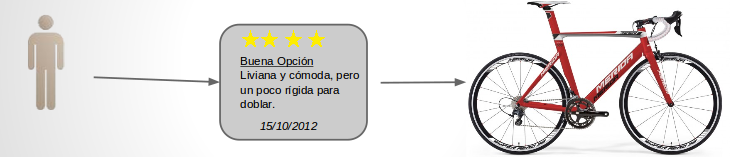
\includegraphics[width=0.8\textwidth,natwidth=610,natheight=642]{biciReview.png}
    \caption{Relación entre usuario, review e ítem}
\end{figure}

La existencia de los reviews en la web es muy importante, ya que dan un panorama socialmente perfeccionado (dado que permiten que no sólo una persona
opine sobre un ítem, lo que da a lugar a muchas evaluaciones y provoca que se acerque al valor real) sobre un ítem, lo que ayuda a 
quienes necesiten una descripción y valoración de los mismos que no provenga de quien los quiere promocionar.

\begin{framed}
\textcolor{red}{Al terminar de leer esta sección, el lector debe entender a que te referís con reviews (en términos generales), que muchas de ellas son publicadas en la web en redes sociales, en sitios de productos etc, y que sirven para ??. Podés agregar algunos ejemplos e incluso imágenes. No queda claro por que en el titulo de la sección dice ``entrecruzadas'', ¿es importante o fue solo una elección al azar?. Para que este se conecte con el que sigue, podés dejar picando algo como ``muchos han intentado procesar automáticamente las opiniones de los usuarios para ... pero eso es muy difícil porque...'' }
\end{framed}


\section{Sistemas de Recomendación}
\label{section:sistemas-de-recomendacion}
\noindent Los sistemas de recomendación son herramientas de software que, en base a un conjunto de ítems (películas, libros, productos, hoteles, etc) e información sobre estos, y un conjunto de usuarios, intentan sugerir ítems apropiados a dichos usuarios. Los sistemas de recomendación se han vuelto una de las herramientas más poderosas para múltiples tipos de aplicaciones web, como comercio electrónico o páginas de noticias. 
\\\\
El desarrollo de estas herramientas, involucra conocimiento en múltiples áreas, como inteligencia artificial, minería de datos, estadística, etc. 
\\\\
Los sistemas de recomendación poseen dos enfoques, el de filtrado colaborativo, y el basado en contenido.
\\\\
Los sistemas de recomendación basados en contenido utilizan un conjunto de informaciones y descripciones de los ítems previamente valorados por un usuario para poder construir un perfil del mismo de manera tal de poder determinar, cuales son sus intereses.

Una vez construido el perfil, pueden procesarse las características de distintos ítems que potencialmente pueden ser recomendados a dicho usuario para determinar si alguno de ellos va acorde al perfil.
\\\\
Los sistemas de recomendación de filtrado colaborativo utilizan la información histórica de cada usuario para intentar encontrar y generar grupos de usuarios con gustos similares. Para lograrlo se compara cada usuario con otro observando qué ítems evaluaron y qué puntajes fueron otorgados. 

De esta forma, si se requiere predecir el interés de un usuario en un ítem, se podrá buscar en dicho grupo de usuarios con gustos similares e inspeccionar aquellos usuarios que hayan realizado un review sobre el ítem.
\\\\
Los sistemas de recomendación de filtrado colaborativo tienen una eficacia superior a los basados en contenido, pero cuentan con una gran desventaja, no permiten predecir intereses para aquellos ítems que aún no poseen evualuaciones, o también para aquellos usuarios que no han evualuado ningún ítem.  A esto se lo llama “arranque en frío”.

\begin{figure}
    \centering
    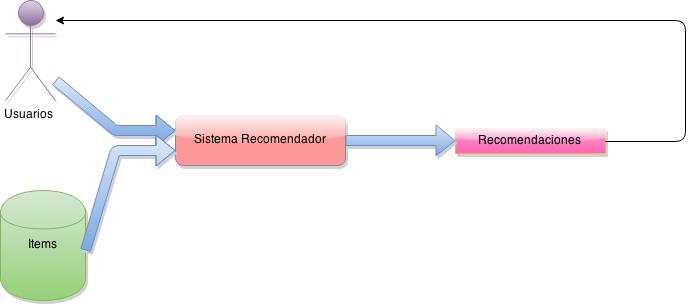
\includegraphics[width=0.8\textwidth,natwidth=610,natheight=642]{recSis}
    \caption{Flujo de un Sistema de Recomendación}
\end{figure}

\section{La web semántica}
\label{section:la-web-semantica}
En sus comienzos en los 90, la web podía verse como un conjunto de sitios web que ofrecían una colección de documentos web interconectados mediante la hipermedia, con el objetivo de comunicar información a los usuarios.
El contenido de esos documentos sólo era generado por el mismo creador y publicador del documento, y los usuarios se limitaban a consumirlo. Por otro lado, era a su vez estático, es decir, se publicaba en la misma forma que se almacenaba y no cambiaba.  
\\\\
Hacia fines de los 90 los sitios web comenzaron a implementar una serie de herramientas (que si bien ya se encontraban disponibles anteriormente no se utilizaban por un problema de performance) que permitieron a los usuarios finalmente participar de la producción del contenido web. Lo que produjo notorios cambios en cuanto a la cantidad de información disponible y proveyó diferentes formas de uso de la web (blogs, redes sociales, canales rss, etc). Más adelante ante la apreciación del pasaje de web estática a una web dinámica, se acuño a esa actual web como web 2.0 y retrónimamente 1.0 a la anterior.
\\\\
Ese cambio provocó un aumento en el tamaño de la web, que se volvió inmenzamente grande, y llevó a la necesidad de implementar tecnologías que ayuden al aprovechamiento de esa cantidad de información. 
Se comenzó entonces a utilizar una serie de frameworks y estándares que permitieron enriquecer (mediante metadatos semánticos y ontológicos dentor de los estándares de la W3C) los datos contenidos en los documentos de manera tal que estos puedan ser consumidos, interpretados y utilizados directamente no sólo por las personas, sino también por las computadoras.
Esto generó que los datos también puedan ser relacionados entre sí, de la misma manera que los documentos son interconectados formando una web de documentos, los datos interconectados forman una web de datos parelela.
Todo este conjunto de actividades frameworks y herramientas forman la ``Web semántica'' que es el puntapié incial para una web mucho más interoperable, lo que permite facilidades para el uso de la web por parte de las aplicaciones y da lugar a otro paso en la evolución de la web, la web 3.0. 
La Web Semántica promete facilitar el desarrollo de la web social y la inteligencia colectiva, a través de mecanismos de clasificación, relación y descripción del contenido de la información publicada mejorando su interoperabilidad. Promete también mejorar la recolección, agregación e integración de datos específicos mediante el uso de agentes de búsqueda automáticos que aprovechan las ventajas.
%Con el correr de los años, múltiples tecnologías se fueron implementando y permitieron el desarrollo de una web mucho más grande y aprovechable...  y esto es unaa referencia a un libro sobre web semantica \cite{Antoniou}

\begin{figure}
    \centering
    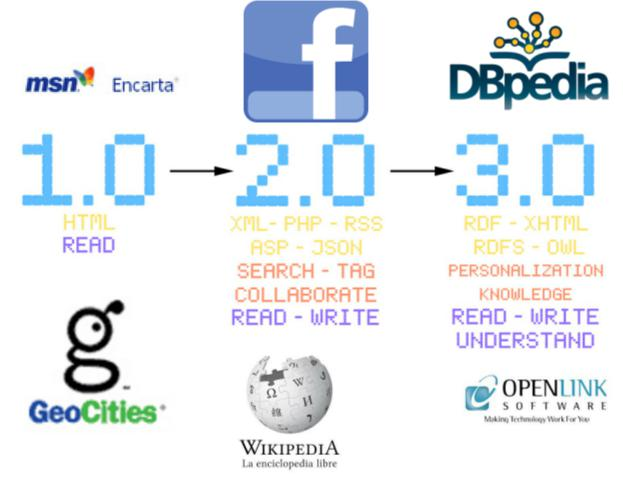
\includegraphics[width=0.8\textwidth,natwidth=610,natheight=642]{webevolve}
    \caption{Evolución de la web}
\end{figure}

\begin{framed}
\textcolor{red}{Al terminar de leer esta sección, el lector debe entender que es la web semántica y a que apunta. Si dejaste picando el tema de automatización en el párrafo anterior, acá se va a imaginar porque hablás de ws. Habla muy bremente de tripletas y meciona RDF. También mencioná linked open data para darle una idea de que la web semantica es una web de datos interconectada. Podés tomar lo que ya escribiste en la propuesta. Ejemplifica con dbpedia o algo asi... En un capitulo mas adelante vas a entrar en detalle en web semantica, rdf, etc. Acá contás solo lo suficiente para que se entienda lo que vas a proponer en la próxima sección}
\end{framed}

\section{Reviews en la web semántica}
\label{section:reviews-en-la-web}

La web 2.0 dio la posibilidad a los usuarios consumidores de la web de generar y publicar contenido en la misma, lo cual cumple con los requerimientos de una plataforma para reviews. Proporciona un entorno para crearlos y publicarlos, lo cual en el caso es una tarea muy sensilla. 
Pero la dificultad de encontrarlos y explotarlos parece ser inversamente proporcional a generarlos. Dado que a mayor facilidad de publicar contenido en la web, mayor se vuelve la inmensidad de la misma y mayor se vuelve la dificultad de encontrar algo dentro de ella.

Veamos dos ejemplos que requieren encontrar reviews en la web:

Imagínense que son ingenieros de Mérida y lanzaron al mercado la bicicleta Reacto 500. Como buenos ingenieros necesitan conocer qué opinan sus clientes, por lo que buscarán reviews en algún motor de búsqueda y luego leerán uno por uno cada review con el objetivo de resumir las opiniones. Humanamente esta tarea demandará mucho tiempo y con un límite corto de cantidad de reviews. 
Ahora peor aún, imagínense que necesitan saber que opina la gente de determinada región (por ejemplo el norte de europa), la tarea de buscar los reviews necesarios se volvería aún más complicada.
Con la posibilidad de contar con una web en la cual los datos son interpretados por las aplicaciones de software y estos a su vez están interconectados, podría crearse una aplicación que pueda automáticamente buscar, clasificar y procesar los reviews para generar automáticamente el resumen.

Ahora bien, si en lugar de requerir reviews de un ítem en particular, se necesitan reviews para una aplicación que recomiende ítems a usuarios, ya no sería una tarea realizable humanamente. Para ello haría falta una aplicación que haga crawling en la web y de alguna manera identifique reviews y a su vez identifique el ítem al cual el review hace referencia. 
Parece algo muy difícil de lograr, salvo que se trabaje sobre sitios conocidos con documentos estructuralmente dominados los cuales se pueda recorrer el DOM automáticamente y acceder a los reviews.
De nuevo, la Web Semántica promete solucionar este problema, con el uso de metadatos que dan información sobre los datos, haciendo que una aplicación pueda fácilmente identificar reviews y navegar por la hipermedia de los datos para conseguir información sobre el ítem y usuario referenciados.

\begin{figure}
    \centering
    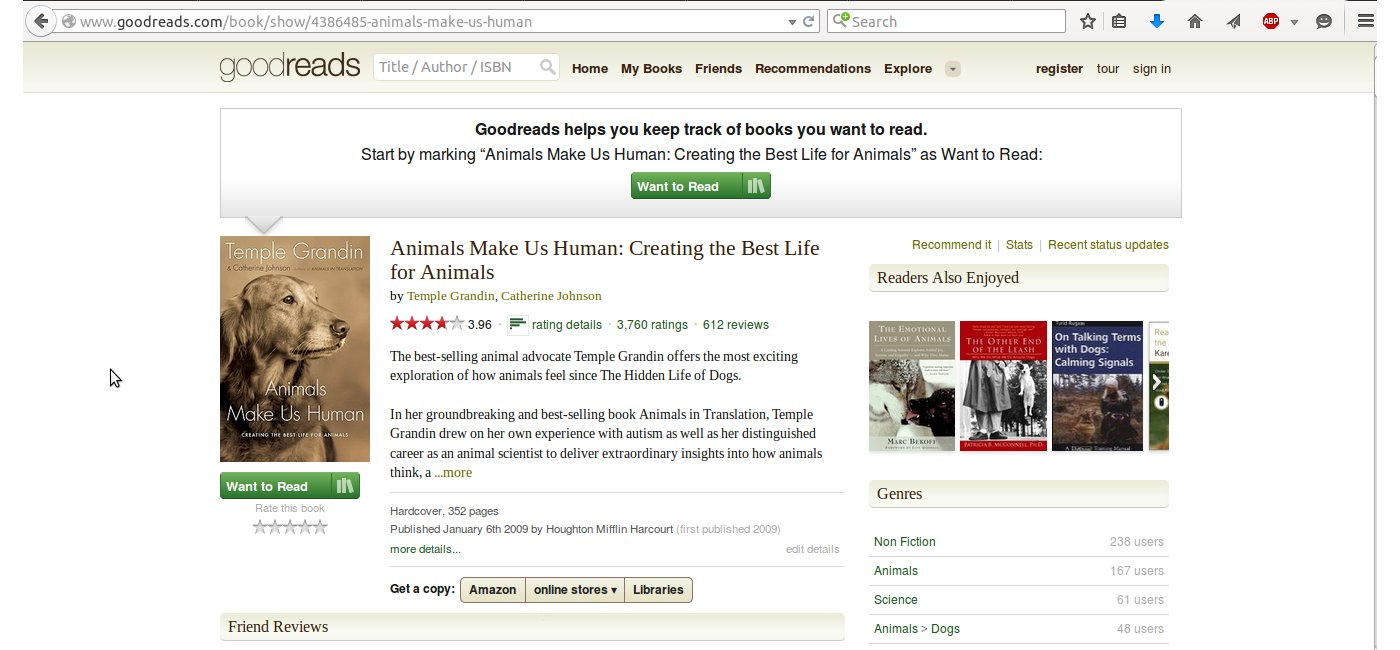
\includegraphics[width=0.8\textwidth,natwidth=610,natheight=642]{semanticwebreview}
    \caption{Ejemplo de review en la web semántica}
\end{figure}

\begin{framed}
\textcolor{red}{Acá es donde presentas el problema a resolver. Ya contaste que son los reviews y por que alguien querría integrarlos. Ya contaste que es la web semántica y linked open data. Ahora tenés que contar que ha habido iniciativas para darle semántica a los reviews y que existen datos; ahora hay una posibilidad de aprovechar esa información. Y ahí decís algo como lo que dijiste al final de la propuesta: \textit{El objetivo principal de esta tesis es evaluar la viabilidad, y entender los desafíos de la utilización de la información contenida en la web semántica en la construcción de sistemas de recomendación. Para eso, y con foco en el caso particular de opiniones de usuarios sobre distintos tipos de recursos se buscará: capturar, extraer, validar calidad, curar, integrar, publicar y explotar los datos disponibles}.}
\end{framed}

\section{Organización}
\label{section:organizacion}

\begin{framed}
\textcolor{red}{ya saben lo que vas a contar; acá les das una idea de como te vas a organizar para contarlo - puede ser algo como lo que está a continuación. Para el caso de estudio podés tomar el texto que escribimos en el articulo}
\end{framed}

El capítulo \ref{chapter:estudio} presenta una aplicación de ejemplo que muestra claramente el problema que se quiere resolver y que servirá como referencia a lo largo de esta tesis. El capítulo \ref{chapter:estrategia} introduce los conceptos de Web Semantica, sus principios y tecnologías y presenta la estrategia de trabajo en términos generales. Los capítulos \ref{chapter:seleccion} a \ref{chapter:explotacion} discuten en detalle cada uno de pasos de la estrategia elegida, aplicándolos al caso de estudio: los reviews en la web semántica. Finalmente, el capítulo \ref{chapter:conclusiones} resumen los resultados observados, saca conclusiones al respecto, y plantea trabajo futuro. El anexo \ref{anexo} presenta una publicación que fue resultado del trabajo efectuado en este trabajo de tesis. 






\chapter{Caso de Estudio}
\label{chapter:estudio}

\chapter{Enfoque General}
\label{chapter:estrategia}

\section{Estrategia propuesta}
Con el fin de crear una aplicación que satisfaga los requerimientos mencionados anteriormente, se debe encontrar
un procedimiento que incluya desde obtener los datos relevantes de la web hasta llevarlos a un estado que permita una 
explotación satisfactoria. 

El procedimiento debería incluir los siguientes pasos  

\begin{description}
\item[Selección de vocabularios ] Tanto la recolección como la publicación de datos en la web semántica involucra la elección del o de los vocabulario/s que mejor modelen el dominio de problema, con la excepción que para su publicación existe la posibilidad de desarrollar uno propio que se ajuste correctamente en caso de que no se encuentre uno existente. 
\item[Recolección  ] Proceso que comprende dos tareas (Búsqueda y Obtención) en el cual se intenta conseguir los datos deseados, los cuales se encuentran dispersos en la web y para ello pueden utilizarse múltiples herramientas y servicios web.
\item[Extracción y almacenaje de los datos] Se le aplica estos dos pasos a los datos crudos obtenidos en la web para poder tener la información semántica y descartar el resto en un formato mucho mejor procesable.
\item[Evaluación de Calidad de los Datos] Se evalúa si los datos poseen la calidad mínima necesaria para crear una aplicación que satisfaga a los requerimientos.
\item[Curado de los Datos] Intentar corregir los problemas de calidad de los datos encontrados en el paso anterior. Siempre y cuando sea posible y viable.
\item[Integración de los datos] Este puede ser el proceso más costoso pero también el más importante, en el cual se intenta unificar e interconectar la información para que pueda ser aprovechable. Existen distintos niveles de integración más simples o más complejos.
\item[Publicación del Dataset Curado] El dataset ya con una calidad teóricamente superior y un estado mucho más aprovechable que el que se encontraba en un primer momento se deja a disposición de todos de forma online.  
\item[Explotación del Dataset] Se construye una aplicación que en base a los requerimientos utilice el dataset. 
\end{description}

\begin{figure}
    \centering
    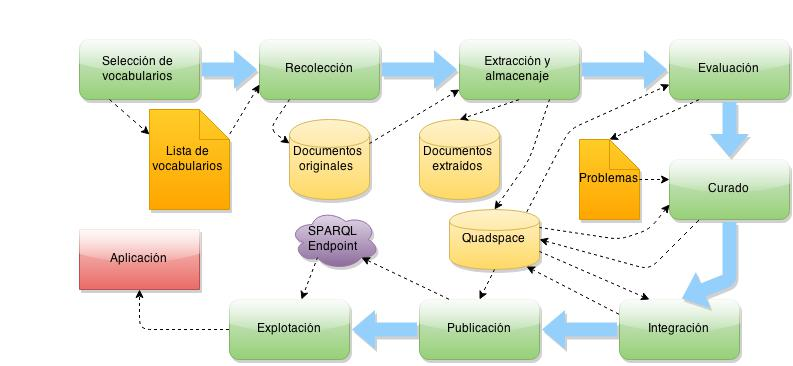
\includegraphics[width=0.8\textwidth,natwidth=610,natheight=642]{proceso}
    \caption{Flujo completo del procedimiento}
\end{figure}

\begin{framed}
\textcolor{red}{acá sería bueno incluir un diagrama que muestre el pipeline. En la lista de arriba con un párrafo se explica cada paso. Luego, en las secciones que sigue se analiza mas cada paso, pero se lo plantea como un problema.. se analizan los retos; entonces los capítulos 4 a 9, explican como los resolviste. Alternativamente, se puede hablar menos acá, solo lo suficiente para que se entienda la estrategia general, y luego en los capítulos 4 a 9 se analiza el problema en detalle y se propone la solución. Con esta ultima forma, todo lo que se refiere a los vocabularios quedaría en el capitulo 4 y no acá. Puede ser mejor.}
\end{framed}

\section{Selección de vocabularios}

\noindent Seleccionar un vocabulario implica analizar varios aspectos del mismo, no sólo su definición e implementación, sino también el uso práctico dado por sus usuarios. 
En primer lugar se debe comprobar que los nombres de las propiedades que posee sean correctamente auto-explicativas. Supongamos por ejemplo que existe un ítem con un rating agregado modelado por una ontología que posee las siguientes propiedades:

\begin{enumerate}
\item minrating
\item ratingValue
\item countRating
\end{enumerate}


\noindent Las dos últimas propiedades resultan fácilmente identificables, ratingValue se trata del promedio de puntaje, y ratingCount 
la cantidad de puntajes que le fueron otorgados, pero la propiedad minRating podría generar distintas formas de interpretación, 
alguien podría suponer que se trata del valor mínimo que fue adquirido por un usuario, o el valor mínimo que un usuario puede 
otorgar. Y muchas veces la documentación de la ontología (si es que existe) no es suficiente.
\\\\
\begin{framed}
\textcolor{red}{Explicar que en realidad uno no elige ``un'' vocabulario sino que la información podría expresarse combinando términos de varios vocabularios. Dejar claro que no es lo mismo elegir el/los vocabulario/s en el que uno va a publicar que decidir cuales son todos los vocabularios que uno va a considerar al buscar información publicada por otros - dar un ejemplo}
\end{framed}

\begin{framed}
\textcolor{red}{Este párrafo que sigue no se entiende; aclarar que sería cubrir las necesidades mínimas de los casos de uso.}
\end{framed}

\noindent Luego se deberá analizar si existen las propiedades para cubrir las necesidades mínimas de los casos de uso. Esto significa que pueda modelar 
toda la información que más adelante será requerida. Por ejemplo, si se quiere construir una aplicación que compare autos, al momento 
de elegir un vocabulario que modele autos, es necesario que contenga ciertas propiedades que puedan expresar información  para determinados 
casos de uso, como comparar cantidad de puertas, lo que requeriría que el vocabulario elegido contenga una propiedad que exprese la cantidad 
de puertas del auto.
\\\\
Es posible que ante una aplicación muy extensa, con casos de uso muy complejos, no se consiga un vocabulario con propiedades tan abarcativas 
que puedan cubrir todos los casos de uso. 

Para esto, se puede aprovechar que las propiedades de un vocabulario, no necesariamente tienen que ser utilizadas estrictamente dentro del mismo.
Lo único que debe respetarse es el dominio y rango de cada una, si no se explicita, puede utilizarse en otros vocabularios.

Goodrelations es un ejemplo del uso de propiedades de múltiples vocabulairos para crear uno nuevo.
\\\\
Y por último se debería intentar buscar ejemplos reales que muestren el uso que le dieron los usuarios a la ontología, para 
determinar qué propiedades están incorrectamente interpretadas o también para los casos donde las propiedades que se encuentren 
en desuso.
\\\\
Con estas precauciones en mente se puede emprender la búsqueda, que podría tener como comienzo búsquedas en  search engines. 
Existen dos buscadores específicos para esta tarea:

\subsection{Linked Open Vocabulary (LOV)}

Proporciona una plataforma técnica de búsqueda y evaluación de calidad sobre un dataset extraído de linked data cloud que contiene descripciones de vocabularios RDFS 
y ontologías OWL. Esas descripciones están en forma de metadatos y pueden ser generados tanto por los autores de los vocabularios como por curadores de LOV.
Posee además de la búsqueda las funciones de estadística o sugerencia.

Actualmente el dataset está integrado por 475 namespaces distintos que contienen una media de 10 clases y 20 propiedades, siendo schema.org el más grande de ellos.

\subsection{Vocab.cc}
Vocabcc es un proyecto opensource que permite a los desarolladores de RDF realizar búsquedas de vocabularios de Linked Data.

Para facilitar la decisión de seleccionar un vocabulario deseado, proporciona además información estadística de cada uno sobre el dataset Billon Triple Challenge (BTCD). 
 Esta información incluye el número de apariciones globales de la URI dada en el BTCD, así como el número de documentos dentro de la BTCD, que contiene el URI dado. Estos números permiten una clasificación de propiedades y clases, respectivamente, con respecto a su uso. También se proporciona información acerca de la posición de una URI dada en estos rankings.

Los desarrolladores pueden buscar las URIs con queries arbitrarias o búsquedas de URIs específicos (prefijos comunes se resuelven automáticamente con datos de prefix.cc).

Para permitir una fácil integración de la funcionalidad vocab.cc, toda la información está disponible como RDF y se puede acceder como Servicio Vinculado.

\begin{framed}
\textcolor{red}{Una vez definidos el/los vocabularios a utilizar, se debe proceder a recuperar información disponible en la web; a eso llamamos ``Recolección''}
\end{framed}

\section{Recolección}
\label{section:recoleccion}
%Como se mencionó antes, la web contiene grandes cantidades de documentos publicados con información semántica. Pero la tarea
de encontrarlos, con el agregado de que sólo una pequeña porción de ellos será relevante para los requerimientos no es trivial
en lo absoluto debido a la inmensidad del universo en el que se encuentran. La forma de llevar a cabo este objetivo está 
atada al hardware disponible, tanto para almacenar los datos, como para el tiempo que va a emplear la ejecución de esta 
tarea. \\
Dado que las bases de datos semánticas sólo almacenan información en forma de tripletas o cuadrupletas, los documentos encontrados 
deberán someterse a un proceso de extracción que seleccione las sentencias HTML y las convierta a alguno de los lenguajes que soportan  
tripletas o cuadrupletas. Para esto existen múltiples herramientas.\\
Una vez transformados los documentos HTML a documentos semánticos puede construirse la base de datos semántica con la información 
recolectada.\\
Como se mencionó antes, la web contiene grandes cantidades de documentos publicados con información semántica. Pero la tarea
de encontrarlos, con el agregado de que sólo una pequeña porción de ellos será relevante para los requerimientos no es trivial
en lo absoluto debido a la inmensidad del universo en el que se encuentran. La forma de llevar a cabo este objetivo está 
atada al hardware disponible, tanto para almacenar los datos, como para el tiempo que va a emplear la ejecución de esta 
tarea.  
\\\\
Dado que las bases de datos semánticas sólo almacenan información en forma de tripletas o cuadrupletas, los documentos encontrados 
deberán someterse a un proceso de extracción que seleccione las sentencias HTML y las convierta a alguno de los lenguajes que soportan  
tripletas o cuadrupletas. Para esto existen múltiples herramientas. 

Una vez encontrados, descargados y transformados los documentos HTML a documentos semánticos puede construirse la base de datos semántica 
con la información recolectada. 
\\\\
Estos son los cuatro pasos necesarios para lograr tener el dataset semántico con el cual se puede empezar a trabajar. Cada uno de ellos 
posee distintas alternativas para su realización, algunas se describirán a continuación 


%\input{opcionesBusqueda}
\\
\input{opcionesDescarga}
\\
\input{opcionesTransformación}
\\
\input{opcionesAlmacenaje} vacio

\subsection{Búsqueda}
%\input{opcionesBusqueda}
\textcolor{red}{OJO: ESTO ESTABA EN EL ARCHIVO busqueda.tex no en el opcionesBusqueda}


La forma de ejecución de esta tarea dependerá de algunos aspectos:
\begin{itemize}
\item Recursos de hardware disponibles

\item Cantidad y calidad de la información requerida

\item El grado de atemporalidad mínima tolerable en los datos

\end{itemize}

El primer paso para realizar la recolección es intentar responder la siguiente pregunta: \textit{¿Dónde encuentro la informanción?}

Una vez seleccionados los vocabularios, se necesitará obtener fuentes de datos que contengan sus datos publicados en los vocabularios previamente seleccionados.
 \\\\
Para lograrlo se podrá utilizar como punto de partida:
\begin{description}
\item[Sitios indexadores:] Son algunos sitios que disponen de un dataset muy grande procesado con documentos indexados, que ofrecen consultar dicho 
dataset a travez servicios web. Generalmente proveen una API donde se pueden consutlar los datos mediante distintos grados de flexibilidad.

Sindice, LOD cloud cache y UriBurner son algunos ejemplos de estos sitios. Se puede utilizar entocnes, dichos servicios web a fin
de obtener una lista de URLs en las cuales se cree que contendrán la información necesaria.

\item[Sitios autoritativos:] Son sitios conocidos que generan información relevante y la publican en las ontologías y vocabularios 
seleccionados. Ejemplos aplicados al caso de estudio podrían ser IMDB (que publica reviews de películas bajo el vocabulario schema), o Rottentomatoes
(que hace lo mismo pero no solo con películas). Se podrán utilizar entonces estos sitios como punto base para un posible crawling.

\item[Catálogos de enpoints:] Son catálogos provistos por algunos sitios que mantienen una lista actualizada de SPARQL endpoints 
junto con el estado de disponibilidad en el que se encuentran. Por ejemplo los sitios http://labs.mondeca.com/sparqlendpointsstatus/ y 
http://www.w3.org/wiki/SparqlEndpoints que este último además provee detalles sobre la información de los mismos.

Consultar estos sitios entonces generará una lista de endpoints SPARQL los cuales se podrían utilizar para pedir la información necesaria.

\item[Volcados de datos:] Son datasets muy grandes que fueron el resultado de un web crawling, los cuales están disponibles para su descarga 
y se pueden utilizar para procesarlos y obtener los datos requeridos. El más importante es http://challenge.semanticweb.org/2014/ .
\end{description}
\subsection{Obtención}

Este paso está directamente relacionado con el anterior, dado que la estrategia de obtención fue planeada con anterioridad, según 
cuál sea la seleccionada, habrá sido la opción ejecutada en el paso anterior.
\\\\
Para este paso se tienen las siguientes estrategias:
\begin{description}
\item[Web Crawling:] Realizar un crawling partiendo de unas pocas URLs seleccionadas en el paso anteiror. Obtenidas de sitios autoritativos.
Existen formas distintas de hacer web craling, dependiendo del nivel de profundidad en el cuál se recorrerá la web, podría también utilizarse los 
sitios indexadores, SPARQL queries, o motores de búsqueda para obtener una lista de URLs que contienen la información deseada, y luego realizar un crawling de profundidad uno sobre cada url.
Hacer crawling con profundidades muy grandes requiere de una algoritmia mucho más compleja para evitar loops, y también de muchos más recursos de hardware, pero se podrá obtener mucha más información.

\item[De-referenciamiento de URIs:] Igual al web crawling, pero exclusivo de documentos semanticos NO embebidos, ya escritos en un formato nativo de la web semántica como RDF, turtle, n-Triples, etc.
Luego la profundidad puede continuarse realizando lo que se llama un ''follow your nose'', que se realiza de-referenciando los documentos que son objeto de la propiedad owl:sameAs, o rdf:seeAlso.

\item[Descarga de las respuestas de las APIs:] Este es otro caso del uso de lso sitios indexadores, SPARQL queries, o motores de búsqueda. Pero en lugar de 
que la información  utilizada sean simpelmente las URL de los documentos, se utilizará también la ifnromación cacheada de dichos documentos y evitarse un crawling.
Como desventaja se puede tener información desactualizada, pero como ventaja se podrá obtener información que ya no esté disponible. Todo dependerá de lo que se busque obtener.
La información obtenida de estas APIs ya debería encontrarse en un formato de la web semántica por l oque no requerirá tampoco una futura extracción.

\item[Procesamiento de grandes volcados:] Este paso requiere de la utilización de recursos minímos de hardware, ya que estos volcados suelen tener volúmenes de varios teras de información, y para procesarlos se requerirá 
de mucha RAM, memoria secundaria y microprocesador.
La idea de este paso es inspeccionar el volcado o bienpara obtener la URL de los documentos con la información deseada, para luego realizar un crawling de profundidad 1, 
o directamente utilizar la información contenida en el volcado.
Esta opción enrealidad es una suma de un paso intermedio con las demás opciones de este paso ya que se estaría realizando el trabajo que hacen los indexadores, que es procesar grandes volúmenes de datos.
\end{description}

\section{Extracción y almacenaje}
\label{section:extraccion}
Una vez que se logró encontrar la información requerida en la web y contener una copia local, se necesita darle un mínimo procesamiento a determinados datos.
Específicamente a aquellos que estén en un formato de información semántica embebida, que requeriran un proceso de extracción para luego ser almacenados en un triplestore.


\subsection{Extracción}

Esto significa, parsear el documento HTML, que como mensionamos anteriormente puede contener información semántica en formato RDF-a, microformatos o microdatos, buscando 
la información semántica para luego generar un documento RDF (o de otro lenguaje de tripletas puro) que represente esa información semántica encontrada en tripletas que puedan ser almacenadas bajo un triplestore.
\\\\
Si bien podría escribirse manualmente un algoritmo que realice esta tarea, existen muchas herramientas que lo hacen, por lo que es recomendable la utilización de alguna de ellas.
\\\\
Los extractores más utilizados son los siguientes:
\begin{itemize}
\item getSchema: Es una herramienta online que se utiliza a travez de una API Restful para extraer documentos con microdatos. Como respuesta se obtendrán documentos semánticos 
con la información extraída en formatos N-Triples, JSON, o N3. 
Es una herramienta rápida y eficaz pero sólo sirve para microdatos.

\item RDF Translator: Funciona también a travez de una API restful, y además de soportar también docuemntos con formato RDF-a, proveé la funcionalidad de transformar los documentos en sentido inverso, 
(de tripletas a información semántica embebida en HTML). 
También está la posibilidad de descargarse la librería y correr el algoritmo localmente.

\item Any23: Una herramienta muy potente y completa que cuenta con una comunidad que lo actualiza constantemente. Al igual que las anteriores se puede utilizar de forma online a travez 
de una API restful. Tiene como ventaja que soporta también microformatos. Es el extractor utilizado por Sindice. 
También está disponible en forma de librería para utilizar localmente.

\item Data Linter:Es una herramienta online que parsea documentos RDF-a, microdatos y JSON-LD.  
Muy útil para analizar documentos, ya que dispone de varias ventajas: 

Presenta la información organizada en tablas anidadas que son mucho más amigables para un análisis humano. 

Posee un mecanismo de inferencia que alerta cuando se viola la sintaxis de los vocabularios.

Como contrapartida, la información retornada por la herramienta es en texto plano. Por lo que no puede ser utilizado en un triplestore.

\end{itemize}

\subsection{Almacenaje}

Con la información recolectada de internet en forma de tripletas (o cuadrupletas) ya puede ser almacenada conjuntamente en un triplestore. 

Se disponen de muchas opciones de triplestores en la actualidad, algunos pagos y otros gratuitos. Cada uno con ventajas en algunos aspectos y desventajas en otros.

Muchos son librerías que forman parte de un framework, además algunos mapean tripletas a otros motores de base de datos como por ejemplo MYSQL o POSGRE.
\\\\
Algunos posibles triplestores pueden ser
\begin{itemize}
\item TDB: Componente del framework Jena, que puede ser accedido mediante linea de comandos o a travez de la API de jena. Almacena tanto tripletas como cuadrupletas, y las almacena en varios archivos donde cada uno indexa los datos de distintas formas. Tiene una muy aceptable performance pero pequeños errores en su uso pueden corromper la información facilmente.

\item SDB: Al igual que TDB es un componente de Jena, pero que no almacena la información como archivos en el disco, sino que mapea los datos a un motor de bases de datos subyacente como MYSQL y POSGRE. Su performance está atada a dicho motor de bbdd subyacente pero por lo general no suele dar buenos resultados. 

\item Sesame triplestore: Componente del framework Sesame, que tiene la opción de almacenar la información en disco o en memoria. Lo que puede significar un improtante beneficio para quienes requieran performance elevada en queries. Soporta no solo SPARQL sino también SeRQL. Tiene además la ventaja de poder integrar Alibaba, que es un mapeador de calses de Java a ontologías RDF.
\end{itemize}

\noindent Aquí hay un par de datos extraídos del paper Chris Bizer, Andreas Schultz. The Berlin SPARQL Benchmark. Int. J. Semantic Web Inf. Syst. 5(2): 1-24 (2009) que habla sobre un benchmark que compara triplestores:

\begin{itemize}
\item To load 100m triples of evaluation data:
 \begin{description}
     \item[Sesame:] 3 days 6 hours
     \item[Jena TDB:] 1.5 hours
     \item[Jena SDB:] 1 day 15 hours
 \end{description}
\item Complex Query Mixes per Hour (rate of query answering -- higher = better) for 1M triples:
 \begin{description}
     \item[Sesame:] 18,094
     \item[Jena TDB:] 4,450
     \item[Jena SDB:] 10,421
 \end{description}
\item Complex Query Mixes per Hour for 25M triples:
 \begin{description}
     \item[Sesame:] 1,343
     \item[Jena TDB:] 353
     \item[Jena SDB:] 968
 \end{description}
\item Complex Query Mixes per Hour for 100M triples:
 \begin{description}
     \item[Sesame:] 254
     \item[Jena TDB:] 81
     \item[Jena SDB:] 211
 \end{description}
\item Simple Query Mixes per Hour for 1M triples:
 \begin{description}
     \item[Sesame:] 38,727
     \item[Jena TDB:] 15,842
     \item[Jena SDB:] 15,692
 \end{description}
\item Simple Query Mixes per Hour for 25M triples:
 \begin{description}
     \item[Sesame:] 39,059
     \item[Jena TDB:] 1,856
     \item[Jena SDB:] 4,877
 \end{description}
\item Simple Query Mixes per Hour for 100M triples:
 \begin{description}
     \item[Sesame:] 3,116
     \item[Jena TDB:] 459
     \item[Jena SDB:] 584
 \end{description}
\end{itemize}
        

No sólo se debería elegir el triplestore en cuanto a su performance, su facilidad de uso y flexibilidad también es un aspecto muy importante a evaluar.

%\input{opcionesDescarga}
%input{opcionesTransformación}
%input{opcionesAlmacenaje}

 

\section{Evaluación de Calidad de los Datos} 
\label{section:evaluacion}
Como sabemos los reviews son creados por usuarios que en su mayoría no están familiarizados con el desarrollo de una 
aplicación, esto causa que una parte muy significativa del contenido publicado no esté de la forma adecuada para ser procesado. 
La falta de calidad en el contenido publicado puede deberse tanto a errores por parte del usuario como por parte del publicador.

El publicador deberá asegurarse que los datos respeten rigurosamente las ontologías en las cuales se publican.
\\\\
El sitio web en el cual el usuario se encuentre realizando el review deberá guiarlo en todo lo posible para lograr que la evaluación
quede en un formato adecuado.

Aunque también existen muchos problemas que no dependen del sitio web, generalmente errores semánticos de calidad, donde lo 
redactado esta hecho de forma inconsistente o insuficiente.
\\\\
Este paso entonces tiene por objetivo encontrar todos los problemas de calidad que pueda haber en el dataset que acaba de 
ser descargado y extraído y que generen inconvenientes para una posterior integración/explotación.
\\\\
La estrategia se divide en dos partes, una formal y otra informal.
\\\\
La formal se encuentra ligada a la detección de errores sintácticos en el dataset, que son generalmente causados por una mala utilización del vocabulario (Aunque también suelen aparecer problemas causados por malas definiciones de los vocabularios)

El ejemplo típico de este tipo de error es el uso incorrecto del dominio o rango de una propiedad. 

Encontrar este tipo de errores no es una tarea demasiado compleja, disponiendo de los vocabularios se puede hacer inferencia sobre el dataset y determinar automáticamente los errores sintácticos.
\\\\
Y luego se encuentra la estrategia informal, que intenta encontrar los problemas semánticos del dataset, para los cuales resulta extremadamente difícil su detección automatizada.

Un ejemplo de este caso es la falta de información precisa necesaria para identificar un ítem, por ejemplo poner ``batman'' como nombre, siendo esta la única forma de identificarlo. Como sabemos batman puede referirse a muchos ítem distintos y se necesita un nombre más preciso para su identificación.
Este problema haría más dificultosa una posible integración, ya que no sería tan simple identificar cuales reviews hablan de los mismos ítems.

Otro ejemplo es el de la inconsistencia en la información provista, si por ejemplo se establece schema:Book como tipo de ítem pero el nombre del ítem es ``Samsung SyncMaster 753s'' claramente es el caso de un tipo incorrecto, ya que hay una propiedad que sólo tendría sentido si se tratara de un schema:Product.
Este último error modificaría el correcto funcionamiento de una posible aplicación resultante además de interferir en la integración. Ya que si esa aplicación por ejemplo, lista reviews según el tipo de ítem, cuando un usuario busque reviews de libros, se encontraría con el review de un monitor.
\\\\
Estos últimos errores suelen ser muy difíciles de encontrar y prácticamente imposibles de detectar mediante búsquedas automáticas.

Para lograrlo se requiere observar humanamente el vocabulario y reflexionar sobre el mismo, deduciendo errores que podrían aparecer, también ayudaría mucho observar resultados de estadísticas sobre el uso de propiedades en el dataset.
\\\\
Existen frameworks para realizar estas operaciones.

%Curado de los Datos\\
En el paso anterior se describieron los problemas en la calidad del dataset que tendrán un impacto en la aplicación resultante, 
o que, podrían limitar o imposibilitar la realización de la misma. Dichos problemas pueden ser muchos, y algunos muy difíciles
de solucionar, será parte entonces del proceso, reconocer aquellos que su resolución sea viable y además encontrar la forma de 
implementarla.\\
Cabe destacar que el proceso de evaluar el dataset en búsqueda de problemas y implementar soluciones es iterativo, debido a que 
una mejora puede conllevar a nuevos problemas.\\
\section{Curado de los Datos}

En el paso anterior se describieron los problemas en la calidad del dataset que tendrán un impacto en la aplicación resultante, 
o que, podrían limitar o imposibilitar la realización de la misma. Dichos problemas pueden ser muchos, y algunos muy difíciles
de solucionar, será parte entonces del proceso, reconocer aquellos que su resolución sea viable y además encontrar la forma de 
implementarla.
\\\\
Cabe destacar que el proceso de evaluar el dataset en búsqueda de problemas y implementar soluciones es iterativo, debido a que 
una mejora puede conllevar a la detección de nuevos problemas.

%Integración de los datos\\
Los datos recolectados fueron generados por distintos usuarios, en múltiples sitios y bajo distintas ontologías y estándares.
Estos aún curados, necesitan un último paso para poder realizar una explotación, y es la integración.\\
Este gran y dificultoso proceso abarca cualquier operación que intente dar una visión más unificada de la información. Este
proceso puede tener distintos niveles y aspectos a integrar, como podría ser por ejemplo, unificar las ontologías de los reviews, o bien
en una nueva ontología de review, o bien en una ya existente, para lograr tener información semánticamente más parecida. Ya 
que este proceso puede ser muy dificultoso, habrá que ver en base a los requerimientos, qué aspectos de los datos se integrarán.\\
Una vez realizada la integración mínima necesaria par also requerimientos, el dataset ya estará listo para su explotación.

\section{Integración de los datos}
\label{section:integracion}
\begin{framed}
\textcolor{red}{Esto va acá o es parte de Explotación?}
\end{framed}

Los datos recolectados fueron generados por distintos usuarios, en múltiples sitios y bajo distintas ontologías y estándares.
Estos aún curados, necesitan un último paso para poder realizar una explotación, y es la integración.
\\\\
Este gran y dificultoso proceso abarca cualquier operación que intente dar una visión más unificada de la información. Este
proceso puede tener distintos niveles y aspectos a integrar, como podría ser por ejemplo, unificar las ontologías de los reviews, o bien
en una nueva ontología de review, o bien en una ya existente, para lograr tener información semánticamente más parecida. Ya 
que este proceso puede ser muy dificultoso, habrá que ver en base a los requerimientos, qué aspectos de los datos se integrarán.
\\\\
Una vez realizada la integración mínima necesaria para los requerimientos, el dataset ya estará listo para su explotación.

\section{Publicación del Dataset Curado}

Existen varias maneras de publicar el dataset, y la elección de una en particular dependerá tanto de para qué se podría utilizar el dataset en el futuro como
de los recursos de tiempo/hardware/económicos que se esté dispuesto a gastar.
\\\\
Una posible solución muy barata y simple es generar un volcado de la base de datos, comprimirlo y subirlo a un hosting de archivos como Mega. Cualquier usuario podría descargarse entonces la base de datos y utilizarla de la forma que más le convenga.
Tendría el problema en ese caso de no serle útil a usuarios con pocos conocimientos sobre esta tecnología, o que no posean demasiados recursos de hardware, o tiempo.

Una solución un poco más costosa es utilizar un servidor (ya sea propio, pago, o simplemente una pc), y crear un SPARQL Endpoint accesible mediante la web.
Esta última opción puede implementarse utilizando algúnas herramientas:
\begin{description}
\item [Fuseki:] SPARQL endpoint que utiliza el protocolo SPARQL mediante HTTP con estilo REST. Tiene una performance aceptable y la ventaja de ser muy sensilla su instalación y puesta en marcha. Se puede directamente utilizar un volcado de TDB.

\item [Virtuoso Server:] Middleware que incluye no solo un endpoint, sino también un motor de base de datos, un server, una aplicación web y todo lo necesario para publicar los datos en la web. Puede ser muy útil pero su instalación y puesta en marcha no es trivial. Y requiere la adquisición de una licencia para su uso.

\item [ARQ:] Componente de Jena que funciona como query engine, y puede ser utilizado para armar el endpoint manualmente, eso singifica realizar a mano la aplicación web.
\end{description}
\section{Explotación del Dataset}
\label{section:explotacion}
\begin{framed}
\textcolor{red}{Acá es donde efectivamente se discute que implica cubrir los requerimientos de la aplicación . Puede ser que acá tambien te refieras a como la forma en la que querés explotar los datos impacta en las fases anteriores. Incluso, habría que pensarlo, en este capitulo tal vez conviene primero hablar de explotación y luego de las otras fases - porque explotación determina mucho que es lo que vas a mirar en las fases anteriores, ¿no?}
\end{framed}

<<<<<<< HEAD
 Finalmente 
=======
\noindent Por último se llega al paso de explotación. 
\\\\
La forma en la que se proceda a implementarlo depende de múltiples factores que dependerán 
de los recursos de hardware disponibles, el tiempo de desarrollo que se deseé emplear y 
la calidad del dataset obtenido en los pasos anteriores.
\\\\
En general, cualquier aplicación resultante será correcta si logra respetar los requerimientos.
\\\\
El único punto a tener en cuenta es el de elegir correctamente un tipo de sistema de recomendación 
de manera que se pueda aprovechar de la mejor forma posible la información existente en el dataset. \\
Por ejemplo, si el dataset no contiene demasiados datos descriptivos de los ítems, no sería 
conveniente utilizar un sistema de recomendación basado en contenido, ya que la aplicación resultante 
no funcionaría de una forma muy útil.
De la misma forma que si dispone una gran cantidad de datos acerca de los autores, debería considerarse 
escoger un enfoque colaborativo para aprovechar de la mejor manera el dataset.
\\
\\
Teniendo eso en consideración, las herramientas/tecnologías/lenguajes/etc utilizados para su 
construcción y desarrollo.
>>>>>>> 49478991009a94744fb73d7dbf44ca15cd0cce27



\chapter{Selección de Vocabularios}
\label{chapter:seleccion}

En la actualidad existen cuatro vocabularios que cumplen los requerimientos mínimos para modelar el dominio de problema planteado.

\subsection{Review Ontology}

RDF Review Vocabulary

También conocido como Review Ontology, es una de las ontologías más antiguas de review, que fue pensada para uso del lenguaje 

RDF y está definido bajo el namespace http://purl.org/stuff/rev\# .

Fue utilizado para la construcción Revyu , y sirvió como guía para otras ontologías.

Consta de tres clases y trece propiedades.

Clases

Comment: Un comentario sobre el review. 

Feedback: Expresa la utilidad del review. 


Review: El review mismo. 


Propiedades


commenter: Especifica el usuario que realizó el comentario del review. Tiene dominio Feedback o Comment y rango foaf:Agent.


Actualmente se encuentra en desuso.


hasReview: Enlaza el ítem evaluado con el review. Su dominio es rdfs:Resource (siendo ésta la clase del ítem evaluado) y su rango es Review. Es una de 
las propiedades principales. 


hasComment: Idem anterior pero con el comentario en lugar del review.

Se encuentra actualmente en desuso.

hasFeedback: Idem anterior pero con feedback en lugar de comentario.

Se encuentra actualmente en desuso.


maxRating: Establece el puntaje máximo que es posible otorgar por un usuario a travez de la propiedad rating. Tiene como dominio 
Review y como rango Literal siendo este último un número positivo. Su ausencia en un review asume su valor por defecto (5). Por lo que 
si bien no es indispensable que esté, se deberá respetar la convención ala hora de generar el rating.



minRating: De la misma forma que el anterior, sólo que establece el puntaje mínimo y su valor por defecto es (1).


positiveVotes: Se refiere a la cantidad de votos positivos que tuvo el review, otorgados por usuarios que lo leyeron y lo encontraron 
útil. SU domino es Review y su rango Literal siendo este último un número positivo.


Se encuentra actualmente en desuso.


rating: Una de las propiedades principales, indica el valor numérico otorgado por el creador del review sobre el ítem evaluado. 
Su domino es Review y su rango es Literal siendo este último un número entre los valores de minRating y maxRating.


reviewer: Especifica el usuario que realizó el review. Tiene dominio Review y rango foaf:Person. 



text: Otra de las propiedades principales, define el texto que describe el sentimento del usuario hacia el ítem. Tiene como 
domino Review y como rango Literal.


totalVotes: Exactamente igual a positiveVotes.


title: El título del review . Tiene dominio Review y rango Literal. Subclase de dc:title


No tiene demasiada utilidad para el caso de estudio y además se encuentra en desuso.


type: Enuncia el tipo de ítem que clasifica taxonómicamente al ítem evaluado. Su domino es rdfs:Resource (siendo ésta la clase del ítem evaluado)  
y su rango no se encuentra especificado. 


Es una propiedad muy útil pero actualmente se encuentra en desuso.


date: Si bien no está definida dentro del vocabulario, es correcto utilizar http://purl.org/dc/terms/date, implica la fecha en la 
que se realizó el review.


\subsection{hReview}

Como se mencionó anteriormente, está establecido por convención, que los microformatos son una forma de publicar información en la 
web semántica, pero al no disponer de namespaces, no pueden ser representados por ninguna ontología o ningún otro lenguaje de la misma. 


Al no poder utilizar ontologías que modelen reviews surgió la necesidad de crear un estándar específico para embeberlos dentro de HTML 
utilizando microformatos.

Dicho estándar se encuentra actualmente en la versión 0.4 y propone el uso de 10 propiedades, que se supone, deberían ser 
suficientes para cubrir todas las necesidades a la hora de generar un review.

summary (opcional): Puede ser el título o nombre del review, o es posible también hacer una pequeña sinopsis del mismo. Se encuentra en desuso.

type (opcional): Representa el tipo de ítem evaluado, pero se encuentra acotado a alguno de estos  product | business | event | person | place | website | url .


También está en desuso.

item: Esta propiedad enuncia toda la información que se crea necesaria para identificar al ítem, mínimamente los atributos nombre, url y foto.


Para lograr bajo una propiedad cubrir todos los atributos, el rango de la misma debería ser un hCard, que luego contendrá las propiedades mínimas necesarias: 
fn, url, photo y cualquier otra que se quiera adicional.

reviewer (opcional): Al igual que ítem, indica todo lo necesario para identificar a la persona autora del review, para lo cual también deberá representarse 
con un hCard. 

dtreviewed (opcional): Se refiere a la fecha en la que fue creado el review. 

rating: El valor numérico con el cual el usuario expresa su satisfacción con el ítem, y está formado por un entero con un solo decimal 
de precisión, que se encuentra dentro del rango 1.0 a 5.0. Dicho rango puede ser alterado con la presencia de las propiedades worst y best 
que restringen el valor mínimo y máximo respectivamente.

descripción (opcional): Establece el valor textual con el cual el usuario expresa su satisfacción con el ítem, creando una 
sinopsis detallada del mismo. 

tags (opcional): Una etiqueta intenta establecer una idea acerque de qué se trata el contenido en una sola palabra para una rápida identificación 
o para mejorar las búsquedas. 

permalink (opcional): Genera una URI que identificará al review creándole una especie de ID, que será útil para los casos donde 
se podría repetir la publicación del mismo. 

license (opcional): Expresa la licencia del review.

El indicador ``(opcional)'' se refiere a si es indispensable para conformar un hReview o no, de manera tal que si no se encuentra una 
propiedad que no está marcada como opcional no podrá ser considerado un hReview.

Cabe destacar que muchas de las propiedades opcionales, podrían ser necesarias para el caso de estudio.

El problema con este vocabulario surge a la hora de trabajar con la información obtenida, que no puede ser representada por ningún otro 
lenguaje de la web semántica, por lo que se vió la necesidad de mapear las propiedades de hReview, a otro vocabulario que sí pueda.

Esto llevó a que en la web donde definen hReview lo consideren compatible con RDF Review Vocabulary, por lo que en Noviembre de 2007 
se creó una herramienta que transforma de uno al otro hreview2rdfxml.xsl,  pero existe un problema con el rango de algunas 
propiedades, por ejemplo reviewer (propiedad homónima en ambos vocabularios, pero una con rango hCard y otra con rango foaf:Person).

En general si bien este vocabulario bien utilizado puede ser efectivo, resulta poco flexible y complciado de manejar por parte 
de quien quiera explotarlos, el motivo por el cual se ha vuelto muy popular es su facilidad para generarlos, dado que 
microformatos es un lenguaje muy sencillo y cualquier persona con un relativamente mínimo ocnocimiento de HTML puede generar 
sin problemas un hReview, teniendo además herramientas online como opción, que generan el código a travez de un formulario. 
Como es el caso de http://microformats.org/code/hreview/creator. 


\subsection{dataVocabulary}
RDF Data Vocabulary

En Mayo de 2009 Google anuncia la introdución de los llamados ``Google Rich Snippets'', estos fragmentos enriquecidos son una convención 
de etiquetas (con soporte para RDFa-lite y microdata) que permitían agregar información útil a los SERP del buscador de Google. De manera tal 
que los datos que contenían estos fragmentos, recibían un tratamento especial.

Sin embargo en el anuncio, Google revela que el soporte se limitó al uso de las clases y propiedades del vocabulario definido en una página 
notoriamente improvisada llamada http://rdf.datavocabulary.org/ . 

En ella se establecían modelos de clases para varios tipos de ítems, tales como Persona, Organización o Producto y también para los Reviews.

La clase Review, quedó definida bajo el namespace http://data-vocabulary.org/Review e incluía las siguientes propiedades:

itemreviewed: Enlace al ítem que está siendo evaluado.

rating: El valor numérico con el cual el usuario expresa su satisfacción con el ítem, tiene como rango un valor numérico bajo la clase 
xsd:string o Rating, y los valores posibles se encuentran en escala de 1 a 5, pudiendo la misma ser alterada con la presencia de las 
propiedades worst y best que restringen el valor mínimo y máximo respectivamente.

reviewer: El autor del review, su rango es dvocab:Person o xsd:string.

dtreviewed: La fecha en la que se realizó el review, no contiene un rango específico pero aclara que debe respetar el formato 
ISO para las fechas.

description: El cuerpo del review que representa el valor textual de satisfacción del usuario con el ítem.

summary: Un resumen corto del review.

Se puede notar la excesiva similitud de este vocabulario con hReview, queda claro que no hubo una intención de innovar algo, 
sino de representar el hReview en microdatos, probablemente por el apuro en la que data vocabulary fue creado.

Vale aclarar que limitar las clases y propiedades posibles en RDFa es básicamente hacerle perder el sentido al lenguaje 
(la decentralización de los vocabularios sobre los términos) haciendo que el lenguaje se utilice como si fuese microformatos, 
pero perdiendo su valor más improtante (la simplicidad) de manera tal que tomó la inflexibilidad de microformatos y la complejidad 
de RDFa.

Más adelante los Google Rich Snippets incluyeron también soporte para microformatos (lo que incluía hReview). 


\subsection{Schema.org}
Schema.org

Luego de los fragmentos enriquecidos y el improvisado vocabulario data-vocabulary creado para soportar los fragmentos, Google 
en conjunto con Bing y Yahoo crearon en el 2011 Schema.org, con el objetivo de obtener un vocabulario más completo y 
organizado para la implementación de los snippets con RDFa y microdata.

Su lanzamiento provocó la inmediata obsoletización de data-vocabulary cuyas clases fueron todas reemplazadas por equivalentes 
dentro de la nueva ontología:

http://www.data-vocabulary.org/Address -> http://schema.org/PostalAddress

http://www.data-vocabulary.org/Geo -> http://schema.org/GeoCoordinates

http://www.data-vocabulary.org/Organization -> http://schema.org/Organization

http://www.data-vocabulary.org/Person -> http://schema.org/Person

http://www.data-vocabulary.org/Event -> http://schema.org/Event

http://www.data-vocabulary.org/Product -> http://schema.org/Product

http://www.data-vocabulary.org/Review -> http://schema.org/Review

http://www.data-vocabulary.org/Offer -> http://schema.org/Offer

Este nuevo vocabulario, recibe constantes actualizaciones, al punto que, al día de la fecha, la ontología cuenta con 946 clases. 

En particular, la clase review, definida bajo el namespace http://schema.org/Review y es subclase de schema:CreativeWork 
que a su vez es subclase de schema:Thing .

Propiedades de Review

itemReviewed	El ítem que está siendo evaluado, tiene rango schema:Thing 

reviewBody 	El valor textual del review de la evaluación, que tiene rango schema:Text 

reviewRating 	El valor numérico del review de la evaluación, que tiene rango schema:Rating 


Propiedades de CreativeWork 

about 	El tema del contenido. Rango schema:Thing. 

aggregateRating 	El promedio de la acumulación de uno o más ratings dentro de un review. Tiene rango schema:AggregateRating 

author 	El autor del contenido. Tiene rango schema:Person o schema:Organization

comment 	Comentarios sobre el contenido. De rango schema:Comment o schema:UserComments.

commentCount 	Cantidad de comentarios. Rango schema:Integer . 

creator 	El autor del contenido. Tiene rango schema:Person o schema:Organization

dateCreated 	Fecha en la que fue creado. Rango schema:Date .

dateModified 	Fecha en la que fue modificado por última vez. Rango schema:Date .

datePublished 	Fecha en de la primer publicación. Rango schema:Date .

publisher 	El publicador. Tiene rango schema:Organization

review 	 	El review sobre el contenido. Tiene rango schema:Review .

text 		Contenido textual. Tiene rango schema:Text .


Properties de Thing

additionalType 	 Tipos adicionales para el ítem que en general son utilizados para especificar tipos externos, como podría ser por ejemplo una película de clase http://schema.org/Movie con el tipo adicional  http://dbpedia.org/ontology/ . Tiene rango schema:URL .

alternateName 	 Especifica un alias. Rango schema:Text .

description 	Una descripción corta del ítem. Rango schema:Text 

name 		Establece el nombre. Rango schema:Text .

sameAs 		Una referencia a una url que desambiguadamente represente al ítem, como podría ser una URL de wikipedia, dbpedia, freebase, etc . Rango schema:URL.

url 		URL del ítem. Rango schema:URL

Unas 60 propiedades de CreativeWork fueron omitidas por no iban al caso ya que sólo tienen razón de ser para otras clases que 
también heredan de CreativeWork. Lo importante aquí es remarcar un par de situaciones interesantes:

=Las propiedades Review:reviewBody, CreativeWork:text y Thing:description podrían contener el valor textual de la evaluación del review semánticamente correcta por la definición de cada una.

=Las propiedades CreativeWork:author y CreativeWork:creator son exactamente iguales. 

=Los valores CreativeWork:dateCreated CreativeWork:dateModified y CreativeWork:datePublished podrían generar confusión. 

=Sería sintácticamente correcto que un Review utilice la propiedad Review .

Más adelante se mostrarán y enumerarán los problemas que estas cuestiones (causadas por el afán de hacer uso de la herencia
lo más posible)  generan. 


\chapter{Recolección de Datos}
\label{chapter:recoleccion}

En la sección \ref{section:recoleccion} se mostraron múltiples alternativas que se dispone 
tanto para buscar y obtener los datos con los que se trabajará a lo largo de todo el desarrollo.
\\\\
A continuación se describe la implementación seleccionada y utilizada para este paso.

\section{Objetivo}
\label{section:recoleccion-objetivo}

\noindent Como se indicó anteriormente la información semántica que va a ser necesaria para construir se encuentra en la web en forma de documentos 
HTML que tienen la particularidad de ser muy efímeros, de manera tal que un documento que poseía datos relevantes a la fecha,
puede al día siguiente, o dejar de estar disponible on-line, o haber cambiado de forma tal que la información de éste ya no es 
relevante, o ya no poseerla. 
\\\\
En la sección 4.2 de \cite{Mendoza2014} se generó una estadística de este caso, donde se estableció que 
en promedio 62\% de los documentos encontrados, continuaban on-line luego de un año, y de estos, sólo un 56\% aún poseían 
datos relevantes. 
\\\\
Si bien armar un dataset con sólo información extraída de los documentos sin descargarlos es posible, la situación anterior 
genera la necesidad de mantenerlos en una copia local para evitar una posible pérdida de los mismos. 
\\\\
El objetivo entonces será armar un repositorio local con los documentos on-line descargados que se cree que tienen la información 
necesaria. 

 
\section{Estrategia}
\label{section:recoleccion-estrategia}

Se optó por la utilización de Sindice como fuente de datos. Dado que contiene indexados suficiente cantidad de documentos de las 
ontologías a utilizar para hacer una prueba del caso.
\\\\
La consulta arrojó: 10.216.632 documentos que contenían la clase purl:Review y 394.533 que contenían la clase schema:Review
Luego en base a que a comienzos del año sindice limitó la paginación de sus consultas a 100, de manera que sólo es posible acceder a 5000 
resultados se planificó la siguiente estrategia:
\begin{enumerate}
 \item Se realizó una consulta de los documentos para cada ontología con los resultados agrupados por dominio (el sitio dueño del documento) ordenada en orden descendiente por cantidad de documentos 
 \item A mano se inspeccionaron y seleccionaron los cuarenta dominios con mayor cantidad de documentos para la ontología que aún conservaban intactos sus documentos
 \item Se ejecutó una consulta para recuperar hasta 5000 URLs de documentos por cada uno de esos 40 dominios.
\end{enumerate}

\noindent Esto generó una lista de URLs a la cuál se le realizó un crawling, para descargar el documento actual de la web por cada uno. Para realizar la descarga se utilizó la librería fluent.

\section{Resultados}
\label{section:recoleccion-resultados}

\noindent Se obtuvieron de las consultas a Sindice 254950 urls de documentos potencialmente contenedores de reviews.
\begin{itemize}
 \item De las 254950 existían 236697 accesibles.
 \item De los 236697 51 documentos tenían una url de más de 255 caracteres por lo que no se pudo almacenar en el disco utilizando la url como nombre del archivo. Y 6 documentos mal formados.
\end{itemize}

\noindent El cuadro \ref{table:ObtencionResults} muestra la estadística resultante de la implementación de este proceso.
\begin{table}[h]
\begin{tabular}{| l | c | }\hline
   Respuesta HTTP & Cantidad de documentos \\\hline
   200 & 236697 \\
   Error sin código & 10026 \\
   408 & 3519 \\
   500 & 2963 \\
   400 & 77 \\
   403 & 25 \\
   Connection reset & 19 \\
   Premature EOF & 8 \\
   Server redirected too many times & 8 \\
   504 & 7 \\\hline
   Total & 254950 \\\hline
 \end{tabular}
\caption{Resultados del proceso de obtención}
\label{table:ObtencionResults}
\end{table}

\include{extraccion}

\chapter{Extracción y Almacenamiento de los Datos}
\label{chapter:extraccion}

Objetivo

Se realizará un proceso de extracción que convierta los documentos con información semántica embebida en documentos HTML en documentos RDF, que luego puedan ser 
almacenados en un triplestore.

La necesidad de tener la información en un triplestore surge de varios puntos:

Tener la información centralizada, así, por cada paso siguiente a realizar, resulte mucho más simple aplicar un mismo proceso a todos los datos.

Tener la información en un mismo lenguaje, por la misma razón que el punto anterior.

Poder realizar queries SPARQL tanto para generar estadísticas como para realizar un curado de la información.

Poder utilizar el motor de inferencias para detectar errores en los documentos.

Estrategia

Se utilizó any23 para extraer el contenido semántico  y generar por cada documento html, un documento en N-Quads.
El motivo de utilizar any23 es que es la única librería que puede ser utilziada en java, y además soporta todos los lenguajes de RDF embebido en HTML.


Luego se utilizó la herramienta RIOT para hacer un merge de todos los documentos nq y generar uno único.

Y po rúltimo se utilizó la herramienta bulkloader para crear una base de datos TDB a partir del archivo nq que contenía todos los documentos nq.


\chapter{Evaluación de Calidad de los Datos}
\label{chapter:evaluacion}

Objetivo:
Encontrar problemas en el dataset que dificulten una posible integración y modifiquen el correcto resultado de una posible aplicación derivada.

Evaluación nº 1 - Vocabularios

Objetivo:
Buscar aquellas propiedades y clases ligadas a recursos relevantes (que estén relacionados con algún review mediante property paths) 
para las cuales no se encuentre representada en ninguna ontología. Y luego verificar que genere algún problema para la aplicación a construir.

Estrategia:
Este primer paso es bastante simple, básicamente se deben conseguir todos los vocabularios utilizados (para saber cuales son estos basta con revisar el namespace 
de los prefijos) y cargarlos en el dataset.
Una vez con los vocabularios cargados se puede realizar una consulta en SPARQL para las propiedades y leugo otra para las clases:

\begin{lstlisting}[frame=single]
SELECT ?c (count (distinct ?o) as ?cantidad)
WHERE{
{
?s <http://local.org/id> ?id .
?s (:|!:)+ ?o .
}UNION{
?s <http://local.org/itemId> ?id .
?s (:|!:)+ ?o .
}
?o a ?c .
FILTER NOT EXISTS{
?c a rdfs:Class.
}
}GROUP BY ?c ORDER BY DESC(?cantidad)
\end{lstlisting}

Luego se puede hacer una consulta igual pero buscando por propiedades.

Resultados:
Los resultados de esta evaluación fueron interesantes. Además de algunas propiedades y clases mal escritas, ya sea por una letra faltante o una minúscula en lugar 
de una mayúscula, se encontró que todas las propiedades utilizadas de la ontología schema estaban incorrectas.

Ninguna de las propiedades encontradas bajo el namespace http://schema.org/ pertenecían a la ontología schema.
Esto se debe a que cada propiedad incluía bajo su path su clase dominio de la siguiente manera: http://schema.org/CLASE/Propiedad .
Por ejemplo:
http://schema.org/Product/aggregateRating en lugar de http://schema.org/aggregateRating

Situaciones como ésta generan problemas cuando se intenta realizar consultas generales. Si por ejemplo se requiriera encontrar todos los aggregateRatings de todos los recursos no alcanzaría con 
una simple querie, habría que realizar tantas queries como clases de la ontología schema existan.

Haciendo un recorrido sobre los datos desde su origen (los documentos html publicados) hasta este punto, se encontró que el problema se 
originó en el proceso de extracción. 
Any23 cuando extrae las propiedades de la ontología schema, modifica las mismas adicionando el nombre de la clase de su correspondiente dominio, provocando que éstas queden incorrectas.

Evaluación nº 2 - Duplicados

Objetivo:
Disponiendo de un gran dataset de información recolectada de la web, un paso muy útil es limpiar aquellos datos innecesarios. 
Este paso consiste en detectar aquellos reviews en el dataset que se encuentren duplicados.

Estrategia:
La forma más sencilla que a cualquiera normalmente se le ocurriría es comparar los reviews todos con todos. Cuyo algoritmo tiene orden cuadrático que para el tamaño del dataset resulta demasiado denso.
El algoritmo que se utilizó fue el siguiente:
1)Por cada ontología de review se escogió arbitrariamente las propiedades más utilizadas y representativas de cada una:

Purl-Review
dcterms:date
rev:text
rev:title
rev:rating

Schema-Review
sorg:datePublished
sorg:description
sorg:name
sorg:author
sorg:reviewBody

Purl-ReviewAggregate
revagg:average
revagg:count
dcterms:date
rev:title

Schema-AggregateRating
sorgagg:ratingCount
sorgagg:ratingValue
sorgagg:reviewCount

Luego se arma en cada ontología un mapa para cada propiedad escogida, que contiene como clave un valor posible existente para esa propiedad, y 
como valor un arreglo con todos los reviews que contiene ese valor para dicha propiedad.
En otras palabras se separaron por cada propiedad, los reviews según su valor para esa propiedad.
Luego se buscaron qué grupos de reviews se encontraban juntos para más de una propiedad mendiante obtener la intersección de ambos conjuntos. Por ejemplo:

Para el valor 4 de la propiedad rev:rating se encuentran {review1, review2, review3}
Y para el valor ``buena película'' de la propiedad rev:text se encuentran {review2, review3, review4}
Entonces la intersección entre el conjunto de reviews para el primer conjunto con el segundo conjunto es {review2, review3}.
Ahora para marcar ese conjunto como posible grupo de duplicados deben cumplir la condición de que, el ítem sobre el cuál el review habla
tiene el mismo nombre en cada uno de los elementos.

Esta comparación se reliza entre todos los conjuntos de reviews de los valores de una propiedad con el resto de los conjuntos de los valores de las restantes propiedades de esa ontología.

Una vez obtenidos los conjuntos de los posibles duplicados se procede ahora sí a analizar minuciosamente los reviews todos con todos pero dentro del conjunto marcado como posible grupo de duplicados
para corroborar.

Resultados:

Se encontraron en total 17343 reviews replicados en un total de 78705 reviews de los cuales.

1009 estaban duplicados dentro de un mismo documento.
64991 estaban duplicados entre distintos documento pero dentro de un mismo dominio
12709 estaban duplicados en documentos pertenecientes a distintos dominios

Ésta es la lista con los dominios a los cuales se le encontraron más cantidad de reviews duplicados:


\begin{tabular}{| l | c | }
Dominio & Cantidad de reviews duplicados \\
4outof10.com &	21582\\
www.superpages.com &	18756\\
www.kollermedia.at &	9864\\
www.realtruck.com &	8372\\
ormigo.com &	8133\\
www.reptilecentre.com &	3440\\
www.querfood.de &	3275\\
www.carsurvey.org &	2766\\
www.chip.de &	1526\\
www.thewinecellarinsider.com &	1491\\
\end{tabular}

Evaluación nº 3 - RDFUnit-Automatizado

Objetivo:
Encontrar todos los problemas sintácticos de los datos relevantes del dataset e identificar cuales pueden representar un problema 
para construir la aplicación.

Estrategia:
El framework crea test automaticamente a partir de las ontologías, buscando una amplia variedad de problemas posibles. Por lo que se 
instaló el framework, se lo proveyó de las ontologías relevantes y se corrieron los test sobre el dataset.

Resultados:

\begin{tabular}{| l | c | }
Total test cases & 2116\\
Succeeded & 2067\\
Failed & 49\\
\end{tabular}

Los tests fallados más relevantes fueron para schema:

\begin{tabular}{| l | c | r | }
http://schema.org/datePublished does not have datatype: http://www.w3.org/2001/XMLSchema\#date & 152138 & 152138\\
http://schema.org/ratingCount does not have datatype: http://www.w3.org/2001/XMLSchema\#decimal & 12509 & 12509\\
http://schema.org/ratingValue has rdfs:domain different from: http://schema.org/Rating & 6198	 & 181178\\
http://schema.org/worstRating has rdfs:domain different from: http://schema.org/Rating & 5867 & 108095\\
http://schema.org/bestRating has rdfs:domain different from: http://schema.org/Rating & 5867 & 122057\\
http://schema.org/aggregateRating is missing proper range & 4984 & 56890\\
http://schema.org/reviewRating has different range from: http://schema.org/Rating & 4095 & 144239\\
http://schema.org/name does not contain a literal value (http://www.w3.org/2001/XMLSchema\#string) & 1310 & 190840\\
http://schema.org/itemReviewed is missing proper range & 1058 & 1505\\
http://schema.org/reviewRating has rdfs:domain different from: http://schema.org/Review & 331	 & 144239\\
http://schema.org/email does not contain a literal value (http://www.w3.org/2001/XMLSchema\#string) & 174 & 174\\
\end{tabular}

Para purl:

\begin{tabular}{| l | c | r | }
http://purl.org/stuff/rev\#reviewer is missing proper range & 83340 & 157004\\
http://purl.org/stuff/rev\#reviewer has different range from: http://xmlns.com/foaf/0.1/Person	 & 73664 & 157004\\
http://purl.org/stuff/rev\#hasReview has different range from: http://purl.org/stuff/rev\#Review & 72398 & 347548\\
http://purl.org/stuff/rev\#title has rdfs:domain different from: http://purl.org/stuff/rev\#Review & 14705 & 104900\\
\end{tabular}

Evaluación nº 4 - RDFUnit-Manual

Objetivo: Correr test manuales en RDFUnit para evaluar el dataset en busca de errores sintácticos no contemplados por los test
automáticos de la evaluación anterior.

Estrategia: Se configuró RDFUnit utilizando patrones del framework para crear tests manuales. Luego se corrió para obtener resultados
de la misma manera que en la evaluación anterior

Resultados:\\
\begin{tabular}{| l | c | r | }
http://purl.org/dc/terms/date has a format different to YYYY-MM-DD & 92580 & 207130\\
http://schema.org/datePublished has a format different to YYYY-MM-DD & 53740 & 144594\\
http://schema.org/publishDate has a format different to YYYY-MM-DD & 50070 & 59825\\
http://schema.org/dtreviewed has a format different to YYYY-MM-DD & 26903 & 26903\\ 
http://purl.org/stuff/rev\#rating is not in the expected range (1-5) & 15319 & 298458\\
http://purl.org/stuff/rev\#rating is not a natural number & 2866 & 301322\\
http://schema.org/ratingValue is smaller than http://schema.org/worstRating & 41 & 108088 \\
http://schema.org/ratingValue is not a natural number & 33 & 60682\\
http://schema.org/ratingValue is not in the expected range (1-5) & 1 & 73090 
\end{tabular}

Evaluación nº 5 - Análisis experto

Objetivo: Encontrar problemas a grandes razgos que son muy difícil de detectar por algoritmos. También indicios indicadores de 
situaciones que lleven a pensar en otras búsquedas de problemas. Esto debería ayudar a entender mejor el dataset para mejorar el manejo 
de los datos en posteriores paso, como el de integración e implementación.

Estrategia: Este último paso de evaluación se comienza con un pantallazo general de cómo está la situación de los reviews. Para esto se pueden analizar las propiedades que contienen los reviews, y luego el valor objeto 
de las mismas. Dado que los problemas sintácticos deberían estar cubiertos en las evaluaciones anteriores, este paso sólo dejaría establecidos
algunos problemas semánticos del dataset, que al ser detectados en base al punto de vista racional humano, resultaría improbable poder encontrar
una solución algoritmica automatizada para el problema.

Primera query:

\begin{lstlisting}[frame=single]
SELECT ?p (count (distinct ?review) as ?cantidad) 
WHERE{
?review a {ReviewClass}.
?review ?p ?o .
}GROUP BY ?p ORDER BY DESC(?cantidad)
\end{lstlisting}

Esta query debería devolver las propiedades que poseen los reviews y la cantidad de reviews que la utilizan para una clase de review dada.

Resultados más improtantes:

Para la clase schema:Review\\
\begin{tabular}{| l | c | }
 Propiedad & Cantidad \\
 http://schema.org/author & 146243 \\
 http://schema.org/datePublished & 144594 \\
 http://schema.org/reviewRating & 143908 \\
 http://schema.org/description & 122519 \\
 http://schema.org/name & 106219 \\
 http://schema.org/reviewBody & 93634 \\
 http://schema.org/publishDate & 59825 \\
 http://schema.org/url & 44905 \\
 http://schema.org/dtreviewed & 26903 \\
 http://schema.org/reviewer & 26903 \\
 http://schema.org/about & 14693 \\
 http://schema.org/keywords & 7119 \\
 http://schema.org/review & 2292 \\
 http://schema.org/itemReviewed & 2071 \\
 http://schema.org/itemreviewed & 67 
\end{tabular}

 Mirando la tabla de resultados, el primer error semántico que salta a la vista son las 2292 propiedades review dentro de un review. 
 Es claramente un error en la producción del documento. 
 Una rápida búsqueda de los documentos con este problema mostró que son 2 los dominios que repiten el error a lo largo de sus documentos
 http://www.ilgiardinodeilibri.it/ y http://www.iplaysoft.com/
 Más en detalle la intención de los autores del documento fue realizar comentarios para los reviews (situación que tiene una solución específica 
 y es el uso de la propiedad <http://schema.org/comments>). 
 La causa principal de que existan errores de este tipo es la ontología schema que aunque no tenga sentido, propone que sea sintácticamente válido
 escribir un review de un review. Dado que la clase Review es subclase de Creative Work, y esta última contiene la propiedad review.
 
 Por otro lado otra propiedad en el listado que llama la atención es description. Analizando la propiedad semánticamente, significaría describir 
 el review en sí mismo, y no el ítem, dado que si ese fuese el objetivo, dicha propiedad estaría en el ítem y no en el review.
 Observando varios de los valores otorgados a esa propiedad en el contexto del review, muestran que se trata de la opinión textual del ítem, 
 para lo cual al igual que en la situación anterior existe una propiedad específica para eso: reviewBody. 
 La causa de que se utilice description en lugar de reviewBody (incluso con mayor frecuencia) proviene de la ontología de data vocabulary, en la cuál 
 como se explicó al principio de la tesis utiliza la propiedad description como propiedad específica para realizar el review textual.
 Puede suceder que sean dominios que migraron sus reviews desde data vocabulary hacia schema y usaron como propiedad equivalente la que 
 era literalmente igual (lo cual es incorrecto). También puede deberse a la custumbre de haber utilizado aquella ontología que hizo que no se le 
 preste atención a este detalle, o simplemente que hayan visto que es también sintácticamente correcto realizar una descripción de un review 
 y creyeron que era correcto utilizarlo para plantear el review textual.
 De cualquier manera la ontología vuelve a generar inconvenientes debido a la jerarquía propuesta (Review hereda description de la clase Thing).
 Vale la pena aclarar que también existe otra propiedad proveniente de Creative Work que es <http://schema.org/text> cuya descripción de la ontología es `
 ``El contenido textual de este trabajo creativo'' la cuál sería sintáctica y semánticamente correcto utilizarla en lugar de reviewBody, aunque 
 no sería la más específica.
 
 La propiedad name, es ampliamente utilizada en los reviews, la descripción de la propiedad en la ontología declara que se refiere al nombre del objeto en cuestión. 
 Claramente no está pensada para un review (Al igual que la anterior se hereda de schema). Esta propiedad tiene sentido para algún objeto con un nombre real, como Teclado Genius L3, o Batman Begins.
 Un análisis en el uso de la propiedad bajo este contexto, demuestra que la intención fue utilizar esta propiedad para proveer un título al review.
 Y al no haber una propiedad provista por parte de la ontología para titular un review el uso de la propiedad name en su lugar si bien 
 es semánticamente incorrecto, no es una mala idea implementarlo.
 
 Puede observarse tambien que se utiliza la propiedad itemreviewed, la cual no existe en la ontología schema, pero claramente es un 
 error de tipeo en un intento de utilizar la propiedad itemReviewed. Éste al parecer es un error sintáctico no cubierto en las evaluaciones 
 anteriores.
 
 Una propiedad curiosa que aparece en el listado es <http://schema.org/about>. Esta propiedad debería describir el tema en el cual 
 se está tratando en el review. Pero un simple vistazo a los valores que toma la propiedad mediante una consulta sparql muestran que 
 el único valor es ``This is required''
 
 Otra propiedad que vale la pena analizar es <http://schema.org/keywords>. Es una propiedad que debería contener palabras que describan al recurso, 
 el recurso en cuestión es el review y no el ítem, por lo que nuevamente nos encontramos con un error semántico en el uso de la propiedad (ya que es sintácticamente 
 correcto utilizarla en un review porque forma parte de la clase CreativeWork), pero no tiene sentido utilizar palabras para describir un review, claramente 
 son palabras que utilizaron para describir al ítem.
 Una observación de los valores verifican lo descripto anteriormente y además muestran que esta propiedad es sólo utilizada en lso reviews por el dominio 
 http://www.kennstdueinen.de/ que además utiliza el idioma danés.
 
 También hay que mencionar la superpoblación de propiedades que establecen la fecha del review: datePublished, publishDate y dtreviewed.
 El motivo por el cual aparecen tres propiedades distintas para referirse a lo mismo es básicamente porque publishDate y dtreviewed no existen bajo la 
 ontología schema. Es el mismo caso que itemreviewed. 
 Es interesante también mencionar que tanto itemreviewed como dtreviewed son propiedades existentes bajo la ontología data vocabulary, 
 por lo que la causa es muy probable que sea a un intento erróneo de migrar el vocabulario de una a otra ontología, o de venir acostumbrado a la 
 ontología anterior y no prestar atención a este detalle.
 En cambio el motivo por el cual muchos dominios optaron por utilizar publishDate en lugar de datePublished, es que hasta fines de 2014, 
 era una propiedad válida que además se encontraba como ejemplo de un correcto uso de la clase Review provisto por parte de la documentación 
 de la ontología. 
 También la misma ontología en su documentación aclaraba que tanto datePublished como publishDate eran indistintas.
 Exactamente esto mismo sucede con la propiedad reviewer, la cual ya no está disponible.
 
 Por último, un vistazo a la propiedad más popular de la clase Review, author, mostró que todos los valores de dicha propiedad están compuestos 
 por un string o más específicamente un Literal. Esto contradice la definición de la ontología schema, tanto la documentación como la implementación, que
 establecen que le rango de la propiedad author es Organization o Person. 
 El asunto más relevante en este caso es entender porqué este error sintáctico de rango de propiedades no fue contemplado en los test 
 automáticos generados por el framework RDFUnit.
 Y la respuesta parece estar en la complejidad con la que establecieron el rango en la definición de la ontología. El extracto de las 
 tripletas relevantes muestran lo siguiente:
 \begin{lstlisting}[frame=single]
 schema:author rdfs:domain schema:CreativeWork .
 _:node1 rdf:type owl:Class .
 _:node2 rdf:first schema:Organization .
 _:node2 rdf:rest _:node3 .
 _:node3 rdf:first schema:Person .
 _:node3 rdf:rest rdf:nil .
 _:node1 owl:unionOf _:node2 .
 schema:author rdfs:range _:node1 .
 \end{lstlisting}
 
 Al parecer la definición del rango de la propiedad author utiliza estructuras de lista y conjuntos que parecen requerir más inferencia de la 
 que el framework RDFUnit puede realizar.
 
 Conclusión: La mayoría de los problemas son ocacionados por la inconsistencia, inestabilidad e incoherencia de la ontología. Principalmente 
 en el afán de hacerla elegante, crearon a Review como subclase de CreativeWork que normalmente suele ser suplerclase de clases que son ítems de reviews
 lo que concluye en una ontología demasiado larga y redundante.
 \\
 \\
 Para la clase purl:Review\\
 \begin{tabular}{| l | c | }
 Propiedad & Cantidad \\
 \verb|http://purl.org/stuff/rev#text| & 207259\\
 \verb|http://purl.org/stuff/rev#rating| & 195005\\
 \verb|http://purl.org/stuff/rev#reviewer| & 154663\\
 \verb|http://purl.org/dc/terms/date| & 146473\\
 \verb|http://purl.org/stuff/rev#title| & 88148\\
 \verb|http://purl.org/stuff/rev#hasReview| & 6424\\
 \verb|http://www.w3.org/2006/vcard/ns#n| & 6424\\
 \verb|http://www.w3.org/2006/vcard/ns#fn| & 6424\\
 \verb|http://www.w3.org/2006/vcard/ns#url| & 6420\\
 \verb|http://www.w3.org/2006/vcard/ns#geo| & 6123
\end{tabular}
\\ 

Los resultados más llamativos son la aparición de propiedades que normalmente se encuentran en el ítem, dado que no tienen sentido para un review
que son hasReview (un review dentro de un review), n (nombre para un review), fn (idem n), geo (posición geográfica de un review).
El hecho de que todas se encuentren en cantidades similares es el gran indicador de que es un dominio repitiendo algún problema a lo largo de sus documentos.
Una inspección de los dominios donde se encuentra cada uan muestra que todas están incluídas en http://hoteles.hotelopia.es y http://hotels.hotelopia.it/
Básicamente el problema es que le asignaron el tipo purl:Review a ítems.
%Estrategia:

%Como base se utilizó el framework RDFUnit que provee funcionalidades que asisten tanto a la búsuqeda de problemas sintácticos como semánticos.

%Para encontrar los errores sintácticos se utilizaró una herramienta del framework que genera test automáticos sobre un vocabulario, y ésto se realizó sobre PURL y SCHEMA.

%RDFUnit también dispone de una serie de patrones de tests que pueden ser aplicados al contexto e implementados, algunos de los cuales pueden ser utilizados para detectar errores semánticos. 



\chapter{Curado de los Datos}
\label{chapter:curado}

\subsection*{Objetivo}
Corregir todos los problemas viables encontrados en el paso anterior que se pueda.

\section{Curado nº 1 - Vocabularios}
\label{section:curado-vocabularios}

\subsection*{Estrategia}
Con una consulta SPARQL, se eliminó la propiedad incorrecta y se agregó la misma en la forma que corresponde.
Todo se realizó con una simple consulta SPARQL

\newpage
\begin{lstlisting}[frame=single]  
DELETE{
  GRAPH ?g {
    ?s ?t ?o .
  }
}
INSERT{
  GRAPH ?g {
    ?s ?p ?o .
  }
}
WHERE{
  SELECT ?g ?s 
  (IRI(CONCAT("http://schema.org/", ?prop)) AS ?p) ?o
  WHERE{
    GRAPH ?g{
      ?s ?t ?o .
      FILTER(REGEX(str(?t), "http://schema.org/*+", "i")).
      BIND(REPLACE(str(?t), '^.*(\#|/)', "") AS ?prop)
    }
  }
}
\end{lstlisting}


\subsection*{Resultados}
Se crearon 2498221 propiedades nuevas de forma correcta correspondientes a cada una de las propiedades incorrectas de la ontología 
schema.

\section{Curado nº 2 - Duplicados}
\label{section:curado-duplicados}

\subsection*{Estrategia}

Se recorrieron todos los grupos de duplicados y se procedió a realizar la siguiente operación:
Se le asignó a cada grupo un id único, al cual llamaremos groupId.
Luego por cada grupo de duplicados se seleccionó de manera arbitraria un representante con un criterio que se describirá a continuación:
Si dentro del conjunto de documentos entre los cuales se encuentran todos los integrantes del grupo de duplicados no existe ninguno 
que contenga un recurso ya elegido anteriormente como representante, se selecciona cualquier recurso de la lista de duplicados al azar.
Caso contrario, se selecciona el primer recurso encontrado en la lista, que pertenezca al documento que ya contiene algún recurso escogido 
como representante.
Esto se realizó de esa forma, para que todos los representantes se concentren en los mismos documentos y no suceda que dos 
documentos idénticos con dos reviews cada uno, no concluyan cada uno con un documento. De esta forma se minimiza la cantidad de 
documentos con reviews en el dataset.
Luego de elegir un representante para el grupo de duplicados, a ese recurso se le asignó una propiedad http://local.org/representantOf y 
como objeto de la propiedad el groupId.
Y para todos los recursos restantes del grupo de duplicados, se les asignó una propiedad http://local.org/duplicatedOf con objeto 
el groupId.

\subsection*{Resultados}

Se asignaron 78705 propiedades duplicatedOf y 17343 representantOf

\section{Curado nº 3 - RDFUnit-Automatizado}
\label{section:curado-automatizado}

Muchos de los problemas detectados por el framework, no otorgaban demasiada información, como por ejemplo
http://schema.org/datePublished does not have datatype: http://www.w3.org/2001/XMLSchema\#date el cual sólo especifica que le 
falta el tipo al recurso objeto, pero no necesariamente significa que esté mal, esto da un indicio de que algo puede andar mal
y será verificado en la consulta manual, en este caso por ejemplo, lo importante es que la fecha tenga el formato apropiado.
Se decidió entonces atacar los problemas más específicos:

\textbf{http://schema.org/ratingValue has rdfs:domain different from: \\\noindent http://schema.org/Rating}

\subsection*{Estrategia}
Primero hubo que investigar, cuáles son todos los dominios para esa propiedad que aparecen en el dataset, para ver si se pueden 
acomodar. Esto se realizó con la siguiente consulta sparql:

\begin{lstlisting}[frame=single]  
select distinct ?dominio (count (?s) as ?cantidad) 
where{
?s <http://schema.org/ratingValue> ?value .
?s a ?dominio .
}GROUP BY ?dominio
\end{lstlisting}

\begin{table}[h]
\begin{tabular}{| l | c |}\hline
 Dominio & Cantidad de recursos \\\hline
 schema:Rating & 120165\\
 schema:AggregateRating & 54815 \\
 schema:Review & 5867 \\
 schema:Product & 331 \\\hline
\end{tabular}
\caption{Dominios encontrados en los recursos con propiedad schema:ratingValue}
\label{table:ratingValueDomains}
\end{table}

En el cuadro \ref{table:ratingValueDomains} se puede apreciar que en la mayor parte de los casos de error, se dieron porque se incluyó la propiedad ratingValue directamente en 
el Review. Ahora surge la necesidad de saber si esos casos donde el Review tiene la propiedad ratingValue, existe una propiedad reviewRating 
con su respectivo Rating.
Se realizó la consulta:

\begin{lstlisting}[frame=single]  
select (count (?s) as ?cantidad) 
where{
?s a <http://schema.org/Review> . 
?s <http://schema.org/ratingValue> ?value . 
?s <http:schema.org/reviewRating> ?rating . 
}
\end{lstlisting}

El resultado fue 0.

Por lo tanto ese problema se solucionó con la siguiente consulta:

\begin{lstlisting}[frame=single]  
DELETE { 
GRAPH ?g{ 
?s <http://schema.org/ratingValue> ?value . 
} 
} 
INSERT{ 
GRAPH ?g{ 
?s <http://schema.org/reviewRating> ?rating . 
?rating a <http://schema.org/Rating> . 
?rating <http://schema.org/ratingValue> ?value . 
}
}
WHERE{
GRAPH ?g {
?s a <http://schema.org/Review> .
?s <http://schema.org/ratingValue> ?value .
}
}
\end{lstlisting}

~\\\\


\textbf{\noindent schema:worstRating and schema:bestRating has rdfs:domain different from: http://schema.org/Rating}

El proceso es igual al anterior y los dominios distintos de rating eran Review, la misma cantidad que en el anterior 5867
\\\\

\textbf{http://schema.org/itemReviewed is missing proper range}

Esta evaluación se refiere a que existen recursos objeto de dicha propiedad, que no tienen un tipo específico. Para ver si 
puede ser resuelto, primer hubo que evaluar qué clase de recursos contienen como objeto, esas propiedades que presentaron problemas.

La evaluación encontró que, todos esos recursos eran URIs de un dominio web 411ca.com para ser derreferenciados. La solución podría haber sido 
descargar dichos recursos y anexarlos a la propiedad, pero lamentablemente dichos recursos no se encontraban disponibles de forma online.
\\\\
\textbf{http://purl.org/stuff/rev\#hasReview has different range from:\\\noindent http://purl.org/stuff/rev\#Review }
En este caso no hay error, el inconvieniente surge porque los recursos de tipo purl:ReviewAggregate utilizan también la propiedad hasReview
que no esta contemplado en la ontología de purl.
\\\\
\textbf{http://purl.org/stuff/rev\#reviewer is missing proper range}
Este caso se da \\\noindent porque se genera un recurso vació, específicamente el reviewer. El reviewer no fue provisto en los documentos originales donde 
se derivó este problema, simplemente establecían el metadato reviewer dejándolo vacío.
\\\\
\textbf{http://purl.org/stuff/rev\#reviewer has different range from:\\\noindent http://xmlns.com/foaf/0.1/Person}
En estos casos analizando qué clase contenian si no era foaf:Person, se observó que la clase era \\\noindent http://www.w3.org/2006/vcard/ns\#VCard.
En todos los casos donde el reviewer no se encontraba vacío, se utilizó un v:card en lugar de un foaf:Person, y esto tiene una explicación, 
y es que al haberse utilizado hreview con microformatos es imposible crear un recurso de esa clase, dado que no se posee un namespace, para que 
eso sea posible, la clase foaf debería encontrarse dentro de los estándares de los microformatos. 
En este caso al no haber alternativa por parte del creador del review, se considera correcto el uso del v-card, en reemplazo de foaf.

\section{Curado nº 4 - RDFUnit-Manual}
\label{section:curado-manual}

\subsection*{\textit{DateProperty} has a format different to YYYY-MM-DD}
Para todas las propiedades que indiquen una fecha, los pasos para reparar este caso son los mismos.

Cuando nos encontramos con este caso, se requiere de otra evaluación para entender cómo encarar el problema. Es una evaluación cuyo resultado
pueda responder la siguiente pregunta:

Si no tiene formato YYYY-MM-DD, ¿Qué formato tiene?

La idea en esta evaluación entonces, es encontrar qué formatos distintos contienen los datos, para poder trasladarlos al correcto.

~\\\\ 
\textbf{Estrategia}\\
Comenzando con la siguiente consulta:

\newpage
\begin{lstlisting}[frame=single]  
SELECT distinct ?date 
WHERE{
?review <http://local.org/id> ?id .
?review {DateProperty} ?date .
FILTER (!REGEX(str(?date), 
"^[0-9]{4}-[0-9]{2}-[0-9]{2}$", "i")) .
FILTER NOT EXISTS{
?review <http://local.org/deplicateOf> ?dup.
}
}
\end{lstlisting}



Esta consulta retorna la fecha de todos los reviews que no estén duplicados y que además dicha fecha no tenga el formato YYYY-MM-DD

Luego observando los resultados manualmente, se presta atención a los primeros resultados y se trata de encontrar con qué patrón están formados 
para luego anotarlo y realizar la misma consulta esta vez filtrando los resultados con dicho patrón. Iterando este proceso hasta que 
queden 0 resultados.

~\\\\\textbf{Resultados}\\

En los cuadros \ref{table:RegExpressionsDate} \ref{table:RegExpressionsDatePublished} \ref{table:RegExpressionsPublishDate} \ref{table:RegExpressionsDtreviewed} se muestran los patrones de expresiones regulares que cubrieron con todos los casos de formatos 
de fechas.
\\
\\
\begin{table}[h]
\begin{tabular}{| l | c |} \hline
Expresión regular & Cantidad de reviews\\\hline
\verb|^[A-z]+ [0-9]{2}, [0-9]{4}$ |& 14715 \\\hline
\verb|^[0-9]{4}-[0-9]{2}-[0-9]{2}.+ |& 17700 \\\hline
\verb|^[0-9]{4}-[0-9]{2}-[0-9]{1} |& 7179 \\ \verb|[0-9]{2}:[0-9]{2}:[0-9]{2}$| & \\\hline
\verb|^[0-9]{2}\\.[0-9]{2}\\.[0-9]{4}$ |& 7172\\\hline
\verb|^[A-z]+ [0-9]{2}, [0-9]{4}.+ |& 5049\\\hline
\verb|^[A-z]{3} [0-9]{1}, [0-9]{4} |& 1847\\\hline
\verb|^[0-9]{2}\\.[0-9]{1}\\.[0-9]{4}$ |& 410\\\hline
\verb|^[0-9]{1}\\.[0-9]{1}\\.[0-9]{4}$ |& 120\\\hline
\verb|[0-9]{2}/[0-9]{2}/[0-9]{2} |& 67\\\hline
\verb|^[0-9]{1}\\.[0-9]{2}\\.[0-9]{4}$ |& 30 \\\hline
\end{tabular}
\caption{Expresiones regulares que representan los formatos de las fechas de la propiedad datePublished}
\label{table:RegExpressionsDatePublished}
\end{table}
\begin{table}[h]
\begin{tabular}{| l | c |}\hline
Expresión regular & Reviews\\\hline
\verb|^[0-9]{4}-[0-9]{2}-[0-9]{2}.+| & 33833\\
\verb|^[A-z]+.[A-z]{2}.[0-9]{4}-[0-9]{2}-[0-9]{2}$| & 33058\\
\verb|^[A-z]{3}\\n.*[0-9]{1}\\n.*[0-9]{4}$| & 25543\\
\verb|^[A-z]{3}\\n.*[0-9]{2}\\n.*[0-9]{4}$| & 17770\\
\verb|^[A-z]+ [0-9]{2}, [0-9]{4}$| & 17069\\
\verb|[0-9]{2}((?!-).)[0-9]{2}((?!-).)[0-9]{4}| & 11720\\
\verb|^[0-9]{2} [A-zéû]+ [0-9]{4}| & 4147\\
\verb|^[0-9]{2}((?!-).)[0-9]{2}((?!-).)[0-9]{4}| & 4093\\
\verb|^[0-9]{2}((?!-).)[0-9]{1}((?!-).)[0-9]{4}| & 2803\\
\verb|^[A-z]{3} [0-9]{1}, [0-9]{4}| & 2783\\
\verb|^[A-z]+ [0-9]{2}[a-z]{2} [0-9]{4}\\.$| & 2058\\
\verb|^[0-9]{2} [A-z]{3} [0-9]{4}| & 1730\\
\verb|^[0-9]{1}((?!-).)[0-9]{1}((?!-).)[0-9]{4}$.| & 1103\\
\verb|^[0-9]{2}-[0-9]{2}-[0-9]{4}$| & 1024\\
\verb|^[A-z]+ [0-9]{1}[a-z]{2} [0-9]{4}\\.$| & 746\\
\verb|^[0-9]{1}((?!-).)[0-9]{2}((?!-).)[0-9]{4}$| & 279\\\hline
\end{tabular}
\caption{Expresiones regulares que representan los formatos de las fechas de la propiedad purl:date}
\label{table:RegExpressionsDate}
\end{table}\\
\\
\begin{table}[h]
\begin{tabular}{| l | c |}\hline
Expresión regular & Cantidad de reviews\\\hline
\verb|[0-9]{2}/[0-9]{2}/[0-9]{2} |& 2511\\
\verb|^[0-9]{2}\\.[0-9]{2}\\.[0-9]{4}$ |& 2207\\\hline
\end{tabular}
\caption{Expresiones regulares que representan los formatos de las fechas de la propiedad publishDate}
\label{table:RegExpressionsPublishDate}
\end{table}\\
\\
\begin{table}[h]
\begin{tabular}{| l | c |}\hline
Expresión regular & Cantidad de reviews\\\hline
\verb|^[0-9]{1}((?!-).)[0-9]{2}((?!-).)[0-9]{4}$| & 14762\\
\verb|^[0-9]{1}((?!-).)[0-9]{1}((?!-).)[0-9]{4}$| & 6358\\
\verb|^[0-9]{2}((?!-).)[0-9]{2}((?!-).)[0-9]{4}$| & 4193\\
\verb|^[0-9]{2}((?!-).)[0-9]{1}((?!-).)[0-9]{4}$| & 1590\\\hline
\end{tabular}
\caption{Expresiones regulares que representan los formatos de las fechas de la propiedad  dtreviewed}
\label{table:RegExpressionsDtreviewed}
\end{table}

Una vez encontrados los patrones, sólo fue cuestión de correr un algoritmo en Java dónde se contemplan todo los patrones y se 
le aplica la corrección apropiada al String y se vuelve a almacenar en el review.
También en varios casos hubo que verificar dónde se encontraba el día y dónde el mes como por ejemplo para casos como éste 
\verb|^[0-9]{2}\\.[0-9]{2}\\.[0-9]{4}\$|
Manualmente se observan los resultados de ese patrón y se puede observar si los primeros 2 números son mes o día.
También hubo casos no tratables como \verb|^[A-z]+ [0-9]{2}| donde no estaba explicitado el año.

\noindent\verb|http://purl.org/stuff/rev#ratingis not in the expected range(1-5)|\\


\subsection*{\textit{RatingProperty} is not in the expected range (1-5)}
Cuando nos encontramos con un review en esta situación, resulta casi imposible incluso manualmente corregir este error con la información 
provista por el review o el documento que contiene el review. Si el rating del review es 7, ¿Cuál es el máximo valor que el autor tenía en mente cuando  
generó la evaluación?. Uno podría pensar que lo más lógico sería 10, pero no se puede saber a ciencia cierta, por lo menos con la información del entorno al review.
Para encontrar la respuesta, se necesita la información de todos los reviews del dominio que contiene el review problemático. 

~\\\\\textbf{Estrategia}\\
Para resolver el problema de rango en los ratings de los reviews entonces, lo primero que hay que hacer es una evaluación, en la cual 
se pueda observar qué valores tomaron los ratings de otros reviews correspondientes al mismo sitio web hosting del review. 
Esto sólo se aplicó par ala ontología purl, dado que apra schema los valores erróneos eran muy pocos y no se justificaba.
Para implementarlo, lo primero que se realizó fue la siguiente consulta

\begin{lstlisting}[frame=single]
 PREFIX xsd: <http://www.w3.org/2001/XMLSchema#> 
 SELECT distinct ?g ?rating ?id 
 WHERE{
 GRAPH ?g{
 ?review <http://local.org/id> ?id .
 ?review <http://purl.org/stuff/rev#rating> ?rating .
 FILTER NOT EXISTS{
 ?review <http://local.org/duplicateOf> ?dup .
 }
 FILTER NOT EXISTS{
 ?rat <http://purl.org/stuff/rev#maxRating> ?best .
 }
 FILTER NOT EXISTS{
 ?rat <http://purl.org/stuff/rev#minRating>  ?worst .
 }
 FILTER ((xsd:integer(?rating) > 5) ||
 (xsd:integer(?rating) < 1)).
 }
 }
\end{lstlisting}

Esta consulta retorna todos las urls de los documentos que contienen el review problemático incluyendo el id del review y el 
rating correspondiente a dicho review.

A partir de esta información, puede obtenerse el dominio de la URL, y almacenarse toda la información en un mapa de Java, donde para cada dominio se 
guarde los valores de los ratings encontrados, y la cantidad de veces que se encontró cada valor de rating.

~\\\\\textbf{Resultados}\\
Los cuadros \ref{table:Chip}, \ref{table:Chronic}, \ref{table:Gamezbo}, \ref{table:Gogobot}, \ref{table:Kollermedia}, \ref{table:Ormigo}, \ref{table:YellowBot} muestran 
los valores incorrectos de rango de reviews encontrados para cada domino y la cantidad de reviews del mismo. Y en base a esos datos 
se pudo inferir el rango correcto para cada uno de los dominios como muestra el cuadro \ref{table:DetectedRanges}




Luego estos resultados se corroboraron manualmente revisando todos los valores que poseía el dominio tanto dentro del rango 1-5 como fuera .
Desde ya que no se puede asegurar la veracidad de los rangos encontrados, dado que por ejemplo, podría suceder que para el dominio 
www.kollermedia.at por mas absurdo que parezca el rango real es 1-11 pero no existe ningún review con el valor 11 en su rating.
Nota: Manualmente se verificó que ormigo poseía simplemente reviews mal generados.

Una vez con estos resultados se puede proceder a corregir los valores de los reviews del dataset.

~\\\\\textbf{Estrategia}\\
Disponiendo de los rango correctos para cada dominio se recorrieron todos los reviews de cada dominio resultante, y se les adicionaron 
las propiedades rev:minRating y rev:maxRating con los valores correspondientes.
Esto no sólo para los reviews con ratings erróneos encontrados en la etapa de evaluación (fuera del rango 1-5) dado que, para los reviews de 
cada dominio con rango encontrado, por más que el rating se encuentre dentro del rango 1-5 y aparente ser correcto,  ya se sabe que dicho dominio se 
maneja con rangos diferentes y el valor real del rating cambiaría (no es lo mismo el valor 3 en un rango 1-100 que en un rango 1-5)

~\\\\\textbf{Resultados}\\
El cuadro \ref{table:DomainRangeCorrections} muestra la cantidad de reviews corregidos de cada dominio habiéndose agregado las 
propiedades necesarias según los rangos inferidos anteriormente.

\section{Curado nº 5 - Análisis experto}
\label{section:curado-analisis}
Propiedades inexistentes o semánticamente incorrectas\\
Son los casos de itemreviewed, dtreviewed, publishDate y reviewBody, ya analizados en la evaluación.
Estrategia: En este caso para todas el procedimiento es exactamente el mismo, y es bastante sencillo, crear una nueva propiedad con 
el mismo sujeto y objeto, pero la propiedad indicada para cada caso y luego borrar la tripleta incorrecta.\\

\begin{table}[h]
\begin{tabular}{| l | c |}\hline
 Propiedad Inexistente & Propiedad correcta \\\hline
 itemreviewed & itemReviewed\\
 dtreviewed, publishDate & datePublished\\
 description & reviewBody\\\hline
\end{tabular}
\caption{Propiedades inexistentes}
\label{table:UndefinedProps}
\end{table}

El Cuadro \ref{table:UndefinedProps} lista las propiedades incorrectas encontradas con su correspondiente indicado.
\\
Comentarios en forma de reviews\\
\subsection*{Objetivo}
Corregir la clase de los recursos que son de tipo schema:UserComments pero fueron clasificados como schema:Review

\subsection*{Estrategia}
Lo que se intentará es cambiar la clase Review del recurso, y transferir todas las propiedades a una equivalente en la clase UserComments.
Por lo que primero se debe inspeccionar qué propiedades contienen dichos recursos.

\begin{lstlisting}[frame=single]
 SELECT distinct ?p
 WHERE{
 ?s a <http://schema.org/Review> .
 ?s <http://schema.org/review> ?review .
 ?review ?p ?o .
 }
\end{lstlisting}

\begin{table}[h]
\begin{tabular}{| l | c |} \hline
Propiedad encontrada & Equivalente en Comment\\\hline
http://schema.org/description & http://schema.org/commentText \\
http://schema.org/reviewBody & http://schema.org/commentText \\
http://schema.org/datePublished & http://schema.org/commentTime \\
http://schema.org/author & http://schema.org/creator \\\hline
\end{tabular}
\caption{Equivalencia de propiedades de la clase Review con UserComments}
\label{table:PropertyEqRevCom}
\end{table}

En el cuadro \ref{table:PropertyEqRevCom} se muestran las propiedades encontradas junto con su equivalente en la clase requerida. 
Entonces simplemente para solucionar el problema alcanza con la siguiente consulta SPARQL:
\newpage
\begin{lstlisting}[frame=single]
 DELETE { 
 GRAPH ?g{ 
 ?s <http://schema.org/review> ?review .
 ?review <http://schema.org/description> ?description .
 ?review <http://schema.org/reviewBody> ?body .
 ?review a <http://schema.org/Review> .
 ?review <http://schema.org/author> ?author . 
 ?review <http://schema.org/datePublished> ?date .
 } 
 } 
 INSERT{ 
 GRAPH ?g{ 
 ?s <http://schema.org/comment> ?review .
 ?review <http://schema.org/commentText> ?description .
 ?review <http://schema.org/commentText> ?body .
 ?review <http://schema.org/commentTime> ?date .
 ?review <http://schema.org/creator> ?author .
 ?review a <http://schema.org/UserComments> .
 }
 }
 WHERE{
 GRAPH ?g {
 ?s a <http://schema.org/Review> .
 ?s <http://schema.org/review> ?review .
 OPTIONAL {
  ?review <http://schema.org/description> ?description . }
 OPTIONAL {
  ?review <http://schema.org/reviewBody> ?body . }
 OPTIONAL {
  ?review <http://schema.org/datePublished> ?date . }
 OPTIONAL {
  ?review <http://schema.org/author> ?author . }
 }
 }
\end{lstlisting}

Por último, el problema encontrado con los objetos de la propiedad author, que deberían ser recursos de tipo schema:Person o schema:Organization, 
necesitan un arreglo.


\begin{table}[h]
\begin{tabular}{| l | c |}\hline
 Valor & Cantidad\\\hline
 0 & 13\\\hline
\end{tabular}
\caption{Rangos incorrectos del dominio www.yellowbot.com}
\label{table:YellowBot}
\end{table}

\begin{table}[h]
\begin{tabular}{| l | c || l | c || l | c |}\hline
 Valor & Cantidad & Valor & Cantidad & Valor & Cantidad\\\hline
 6 & 1 & 48 & 6 & 79 & 86\\
 8 & 2 & 55 & 7 & 72 & 81\\
 9 & 1 & 54 & 15 & 73 & 70\\
 19 & 1 & 53 & 5 & 74 & 72\\
 25 & 1 & 52 & 12 & 82 & 136\\
 27 & 1 & 59 & 8 & 85 & 120\\
 29 & 1 & 58 & 18 & 84 & 92\\
 31 & 1 & 57 & 11 & 87 & 128\\
 30 & 1 & 56 & 19 & 86 & 91\\
 34 & 1 & 63 & 25 & 81 & 97\\
 33 & 2 & 62 & 23 & 80 & 117\\
 38 & 1 & 61 & 12 & 83 & 115\\
 36 & 3 & 60 & 12 & 96 & 34\\
 37 & 1 & 68 & 62 & 93 & 52\\
 42 & 1 & 69 & 34 & 92 & 68\\
 43 & 3 & 70 & 50 & 95 & 49\\
 40 & 1 & 71 & 62 & 94 & 58\\
 46 & 1 & 64 & 24 & 89 & 98\\
 47 & 4 & 65 & 39 & 88 & 103\\
 44 & 1 & 66 & 35 & 91 & 91\\
 45 & 4 & 67 & 32 & 90 & 93\\
 51 & 9 & 76 & 82 & 100 & 101\\
 50 & 10 & 77 & 82 & 98 & 11\\
 49 & 8 & 78 & 81 & 99 & 8\\
 48 & 7 & 75 & 73 & 97 & 27 \\\hline
\end{tabular}
\caption{Rangos incorrectos del dominio www.chip.de}
\label{table:Chip}
\end{table}
 
\begin{table}[h]
\begin{tabular}{| l | c |}\hline
 Valor & Cantidad\\\hline
 0 & 5\\\hline
\end{tabular}
\caption{Rangos incorrectos del dominio www.gamezebo.com}
\label{table:Gamezbo}
\end{table}

\begin{table}[h]
\begin{tabular}{| l | c |}\hline
 Valor & Cantidad\\\hline
 0 & 1\\\hline
\end{tabular}
\caption{Rangos incorrectos del dominio www.gogobot.com}
\label{table:Gogobot}
\end{table}

\begin{table}[h]
\begin{tabular}{| l | c |}\hline
 Valor & Cantidad\\\hline
 0 & 9\\
 -1 & 24\\\hline
\end{tabular}
\caption{Rangos incorrectos del dominio www.ormigo.com}
\label{table:Ormigo}
\end{table}

\begin{table}[h]
\begin{tabular}{| l | c |}\hline
 Valor & Cantidad\\\hline
 0 & 17\\
 6 & 391\\
 7 & 776\\
 8 & 851\\
 9 & 497\\
 10 & 101\\\hline
\end{tabular}
\caption{Rangos incorrectos del dominio www.chroniclesofchaos.com}
\label{table:Chronic}
\end{table}

\begin{table}[h]
\begin{tabular}{| l | c |}\hline
 Valor & Cantidad\\\hline
 6 & 19\\
 7 & 26\\
 8 & 26\\
 9 & 7\\
 10 & 7\\\hline
\end{tabular}
\caption{Rangos incorrectos del dominio www.kollermedia.at}
\label{table:Kollermedia}
\end{table}

\begin{table}[h]
\begin{tabular}{| l | c | r | }\hline
 Dominio & Rango mínimo & Rango máximo \\\hline
 www.gamezebo.com & 0 & 5 \\
 www.yellowbot.com & 0 & 5 \\
 www.chroniclesofchaos.como & 0 & 10 \\
 www.kollermedia.at & 1 & 10 \\
 www.chip.de & 1 & 100 \\\hline
\end{tabular}
\caption{Rangos detectados automáticamente para cada dominio}
\label{table:DetectedRanges}
\end{table}

\begin{table}[h]
\begin{tabular}{| l | c |}\hline
 Dominio & Cantidad de documentos \\\hline
 www.gamezebo.com & 3905\\
 www.yellowbot.com & 8955\\
 www.chroniclesofchaos.como & 4966\\
 www.kollermedia.at & 9968\\
 www.chip.de & 13751\\\hline
 Total & 41545\\\hline
\end{tabular}
\caption{Cantidad de correcciones de rango de ratings por dominio}
\label{table:DomainRangeCorrections}
\end{table}

\subsection*{Estrategia}
Primero es necesario saber qué representan esos textos utilizados como objeto de author, una observación de esos valores mostró que 
en su gran mayoría representan usernames dentro de la página publicadora, y el resto nombre y apellido.
Esto genera un problema a la hora de llevar a cabo la corrección, ya que de por sí, schema:Person utilizada una propiedad para el nombre (givenName) 
y otra para el apellido (familyName), y no hay una propiedad específica para un username, aunque existe la propiedad alternativeName que 
se utiliza para los nombres que no encajen en las demás propiedades que podría ser utilizado para el username.
Pero cómo saber automáticamente cuando es un username, y cuando es un nombre completo, y más aún, en los nombres completos, cómo saber cuál es el nombre y 
cuál es el apellido?.
Esto no puede ser automáticamente resuelto, por lo que se optó por incluir a todos (tanto usernames como nombres completos) dentro de la propiedad name, heredada de 
schema:Thing.
Entonces como procedimiento final, se cambio el objeto de las propiedades author, por un recurso de tipo Person, con una propiedad name conteniendo 
como objeto el antiguo valor de author. Realizado con la siguiente consulta SPARQL:\\
\begin{lstlisting}[frame=single]
 DELETE { 
 GRAPH ?g{ 
 ?s <http://schema.org/author> ?author .
 } 
 } 
 INSERT{ 
 GRAPH ?g{ 
 ?s <http://schema.org/author> _:foo .
 _:foo a <http://schema.org/Person> .
 _:foo <http://schema.org/name> ?author .
 }
 }
 WHERE{
 GRAPH ?g {
 ?s a <http://schema.org/Review> .
 ?s <http://schema.org/author> ?author .
 }
 }
\end{lstlisting}

\chapter{Integración de los Datos}
\label{chapter:integracion}

Como quedó explicado en la sección estrategia, integración comprende los procedimientos que se realizan con el objetivo de obtener una
visión más unificada del dataset.
Esto puede significar, modificar los datos y ontologías y también agregar información faltante en los ítems/reviews.
Este es el paso más importante de todo el proceso y la posibilidad de conseguir realizar una aplicación correcta que satisfaga los requerimientos
depende del éxito obtenido en el mismo.
En base a los requerimientos establecidos, se pueden pensar en distintos procedimientos que son necesarios para poder explotar los datos
correctamente:
\\
\\
Unificación de vocabularios: En el primer paso del proceso se realizó una selección de los vocabularios con los que se trabajará, 
estos vocabularios modelan el mismo dominio de información pero muchas veces de forma distinta. Explotar información modelada de 
diferentes maneras puede resultar innecesariamente engorroso, y también para quienes en un futuro quieran hacer uso del dataset (ya que
deberán consutlar la información previamente conociendo todas las ontologías de review existentes).\\
Unificación de autores: Es muy importante para lograr cumplir el objetivo de los requerimientos que si dos reviews distintos fueron 
generados por el mismo autor, esto quede explícitamente asentado, para poder realizar los algoritmos de recomendación.\\
Unificación de ítems: El paso más difícil y más importante, si un ítem está modelado dos veces de forma distinta debería saberse que 
se trata del mismo.\\
Unificación de tipos de ítems: Esto es muy útil para darle más posibilidades a la aplicación, y es agrupar los ítems según su tipo 
(Libro, película, Hotel, Auto, etc), de manera que por ejemplo si un usuario quiere que le recomienden un libro, la aplicación sólo 
le ofresca libros. Para la ontología schema, esto puede ser más sensillo dado que los ítems ya se encuentran con su tipo identificado con 
la clase, en el caso de libro, sería cuestión de buscar ítems con la clase schema:Book. El problema es que esto puede no ocurrir siempre, 
Un libro, puede estar clasificado como schema:Product, por lo que necesitaría que también lo clasifiquen como Book.\\
\\
\\
Por razones de que la tesis ya cubrió el desarrollo suficiente, sólo se intentarán implementar los puntos 1 y 4 de la integración. Ya que 
los otros dos son demasiado abarcativos y pueden requerir demasiado trabajo.\\
\\
Unificación de vocabularios\\
\\
Objetivo: Conservar los reviews del dataset en una única ontología. Lo que simplificará las búsquedas, agregaciones y otras operaciones.
Además de contener datos semánticamente más parecidos. Y también facilitará la comprensión del dataset a quienes quieran hacer uso del mismo
en un futuro (ya que sólo deberán concentrarse en una sola ontología)
\\
Estrategia: Deberá como primer paso realizarse una selección de vocabulario, en la cual se escoja uno para que quede como el único en el dataset.
En este caso de estudio el vocabulario elejido es Review Ontology, ya que todas sus propiedades son suficientes para cumplir los requerimientos y 
este es mucho más simple, lo que facilitará su utilización. El vocabulario de schema poseé demasiadas propiedades que son irrelevantes para este caso de estudio. 
Además vale la pena recordar los problemas encontrados en el capítulo evaluación causados por la ontología.
Como segundo paso, buscar para cada propiedad de schema:Review utilizada en el dataset su contraparte en la ontología purl.\\
La equivalencia entre las propiedades ya fueron realizadas en el capítulo de selección de vocabularios. Pero sólo fue realizado con las propiedades 
relevantes al caso de estudio. Las siguientes propiedades (que valga la redundancia son irrelevantes al caso de estudio) fueron utilizadas dentro del dataset, y 
no se estableció su equivalente en el otro vocabulario:
http://schema.org/about y http://schema.org/keywords. 
Si bien, la falta de estas propiedades no impactará sobre la aplicación final, es conveniente no perder datos para la publicación del dataset, ya que 
a alguien podría resultarle útil. 
En la etapa de evaluación se observó que la propiedad about, se utilizó en el dataset sólo para poner contener el valor ``This is required'' en todos los casos. 
Por lo que no incluir esta propiedad en el dataset no producirá una pérdida de información.
Y la propiedad keywords puede ser reemplazada por http://purl.org/dc/terms/subject. Ya que en la documentación de dublin core, proponen la utilización de esta propiedad 
utilizando keywords.
El caso de reviewRating, que tiene como objeto un schema:Rating, no puede ser explicitamente reemplazado, ya que esa propiedad 
sólo es utilizada para desacoplar el rating del review, situación que no se da en la otra ontología. Pero las propiedades dentro del rating se encuentran todas 
con su equivalente en purl, por lo tanto no causará ningún problema.
Por último, schema:Person que es rango de la propiedad author, debería ser mapeado a foaf:Person que es objeto d ela propiedad reviewer. 
El problema se encuentra en lo analizado en la etapa de curado, que se observó que los nombres de los autores podía ser nomrbes completos o usernames. 
Y no existe una propiedad dentro del vocabulario de foaf:Person que sea tan genérico como para contemplar todo slos casos posibles, como sí existe en vCard.
Además de que todos los previos valores de reviewer están conformados por un vCard, como también ya se analizó en la etapa de curado.
Por estos motivos se determinó continuar utilizando vCards en lugar de recursos de tipo foaf, y dichos vCards utilizarán la propiedad
fn (que contempla todos los casos mencionados).
Finalmente el mapeo de propiedades quedaría:\\
\begin{tabular}{| l | c |}
Propiedad schema & Propiedad de reemplazo\\
name & title \\
reviewBody & text \\
datePublished & dc:date \\
author & reviewer \\
ratingValue & rating\\
bestRating (reviewRating) & maxRating\\
worstRating (reviewRating)& minRating\\
url & vcard:url\\
keywords & dc:subject\\
name (author) & vcard:fn (reviewer)\\
comments & hasComment\\
author (comment) & commenter \\
text (comment) & commentText 
\end{tabular}

	
\chapter{Publicación del Dataset Curado}
\label{chapter:publicacion}

Para este paso, se escogió en un primer lugar el aprovicionamineto de un servicio web para ser accedido públicamente. Esto beneficia 
a los usuarios que requieran hacer un uso inmediato y simple de la información contenida. Ya que si se decidiera proporcionar un 
volcado de datos, el usuario deberá tener conocimiento de la manupulación del disco, así como recursos de hardware y tiempo de configuración.\\
\\
Para proceder con la publicación del dataset de la forma mencionada, el motor que se optó por utilizar es Fuseki, ya que proporciona un
medio de implementación extremadamente sencillo, debido a que funciona perfectamente en conjunto de un dataset TDB, que es con el que 
actualmente se cuenta. \\
Fuseki además, tiene la ventaja de ser fácilmente configurable, y no requiere instalación. En el caso de haber elegido otros motores, 
habría que haber hecho una conversión del dataset para obtenerlo en un formato adecuado, además del esfuerzo necesario para instalar y configurar 
toda la aplicación.\\
\\
Por otro lado se consideró también que podría existir la necesidad por parte de algunos usuarios (la minoría), en hacer un uso más complejo del 
dataset (recordar que la utilización de endpoints sparql tiene sus restricciones), para lo cual requerirían manipular el dataset completo 
por su cuenta.\\
Resolver esta situación, no representó casi inconveniente, debido a la alta capacidad de compresión de datos que poseé una base de datos TDB, 
que pasó de 8,4Gb a 1,0Gb. Dicho dataset con esas características puede ser fácilmente publicado para una posible descarga muy fácilmente. 


\chapter{Explotación del Dataset}
\label{chapter:explotacion}

En la sección \ref{section:explotacion} se habló de la elección de un sistema de recomendación, previo 
a la construcción de la aplicación con el objetivo de aprovechar lo más posible la información.\\
\\
Hasta aquí se generó un dataset curado, que en la sección de integración por cuestiones de complejidad 
(e incluso de posibilidad) no se realizó la integración tanto de los autores, como de los ítems.

Dado que no se dispone de ninguna propiedad para determinar que tanto dos autores son el mismo o dos ítems son el mismo 
resulta inadecuado la utilización de un sistema de recomendación de filtrado colaborativo.

Esto también puede incluir a los sistemas de recomendación basados en contenido, porque también hacen uso de 
un perfil de usuario que requiere mucha cantidad de información de cada uno para su construcción.
\\\\
Es por eso que sólo resta la implementación de un sistema de recomendación no personalizado.

De manera que los rankings generados por la aplicación, van a ser idénticos para cualquier 
usuario que lo solicite.
\\\\
Se generó entonces una aplicación que hace uso del dataset publicado en el capítulo anterior, 
cumpliendo con los requerimientos planteados en la sección \ref{section:caso-de-estudio}.

La figura \ref{figure:explotacion} muestra un diagrama de la arquitectura de la aplicación compuesta por tres capas:

\begin{figure}
    \centering
    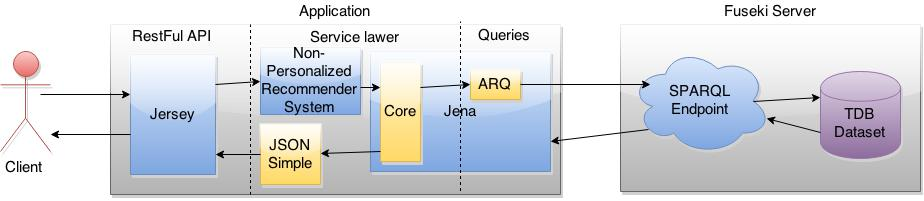
\includegraphics[width=0.8\textwidth,natwidth=610,natheight=642]{explotacion}
    \caption{Arquitectura de la aplicación}
    \label{figure:explotacion}
\end{figure}

\begin{enumerate}
 \item API Restful: Que provee una API mediante la utilización del framework Jersey. Esto evitó 
 que se requiera utilizar una interfaz gráfica que no cumple ningún aporte a los objetivos de esta tesis.
 \item Service: Que proporciona la funcionalidad de la aplicación, generando la estructura de los 
 rankings en el sistema de recomendación, para luego utilizar el framework Jena que modela y proveé la información 
 solicitada por el sistema. 
 
 También posee una librería que mapea la información otorgada pro Jena a Strings JSON que pueden ser 
 devueltos por la API.
 \item Queries: Por último se encuentra la capa queries, que se encarga de obtener los datos del dataset 
 mediante consultas SPARQL generadas por la librería ARQ del framework Jena. Dicha capa será la encargada 
 de interactuar con el SPARQL Endpoint disponible por el servidor Fuseki.
\end{enumerate}

\part{Conclusiones}

\chapter{Conclusiones y trabajo futuro}
\label{chapter:conclusiones}

\noindent Se demostró cómo puede hacerse uso de las tecnologías, frameworks y estándares de la Web 
Semántica para explotar las contribuciones de los usuarios a lo largo de toda la web dentro 
del marco de los Sistemas de Recomendaciones.
\\\\
A partir de todo el proceso se pueden distinguir dos actores que participan en la publicación 
de reviews en la web semántica, el usuario que genera la información y el desarrollador
del sitio que proveé al usuario la plataforma para hacerlo.
\\\\
La importancia entonces de la existencia de vocabularios expresivos, concretos y precisos 
resulta fundamental para ayudar a estos dos a publicar la información correctamente, ya que 
se demostró que a partir del paso Evaluación, la incorrectitud en la información publicada 
crea grandes problemas que resultan muy complicados de resolver, al igual que se demostró 
que muchos de los errores son muy influenciados por los vocabularios.
\\\\
Aún con vocabularios completos, correctos y precisos, continuarían presentándose dificultades en 
el paso de Integración, ya que es muy dependiente de la relación entre los datos publicados 
por distintos usuarios.

Intentar integrar ítems y autores parece ser entonces una tarea que va de extremadamente compleja 
a imposible, dado que la mayoría de los reviews poseén de información de los autores sólo un username, 
en lugar de un identificador global como podría ser una dirección de email.

También ítems, que tampoco poseén identificadores globales, sino nombres escritos en 
distintos formatos.

Esto parece tener origen en la naturaleza decentralizada de la web semántica, que otorga 
a los usuarios la libertad de generar recursos sin límite.

La solución no parece encontrarse por el camino de la centralización, como fue planteado en \cite{Heath2006J} cuya
aplicación resultante terminó siendo obsoleta,
sino con la estandarización más restrictiva en vocabularios y propiedades, intentando 
llevar a los usuarios a la utilización de esos tan necesarios identificadores.
\\\\
Por otro lado se pudo observar la preferencia de los desarrolladores de sitios a la utilización de 
formatos de código semántico embebido en HTML, en lugar de documentos RDF puros. Aunque cada uno de 
los formatos poseé ventajas y desventajas para dicho desarrollador del sitio, se notó que uno de ellos 
(microformatos) sólo contnía desventajas desde el punto de vista del desarrollador de la aplicación 
semántica. 

Dicha conclusión  se obtiene de verificar que la calidad de los ítems escritos en microformatos del 
dataset es muy baja, ya que sólo poseén como información un nombre en la mayoría de sus casos.

Esto se debe a que no se disponen de namespaces para la utilización de ontologías que permitan 
la utilización de propiedades descriptivas necesarias, y sólo cuenten con el uso de V-Cards.

El punto de vista del desarrollador de aplciaciones semánticas por supuesto que no suele ser tenido 
en cuenta por el desarrollador de sitios, que la mayoría de las veces opta por el uso de 
microformatos por su simplicidad.
\\\\
A pesar de los problemas mencionados, se alcanzó el objetivo de construir un sistema de recomendación, 
dondé se produjeron satisfactorios resultados en los puntos de evaluación y curación. 
Y dicha construcción demostró cómo puede ser necesarios combinar vocabularios (como se vió en 
el capítulo \ref{chapter:integracion} que se aprovechó la simplicidad y correctitud de la 
Review Ontology para los reviews para los ítems de schema), y mostró interesantes usos 
de la minería de datos para el proceso.

También mostró la necesidad de conocer las distintas herramientas y aplicaciones como Sindice 
o RDFUnit, que aportan mucho al proceso, también de la necesidad de conocer la naturaleza de 
los datos con los que se trabaja.
\\\\
Quedan entonces planteados, desafíos en varios de los puntos de este trabajo, comenzando con 
la proposición de estándares o soluciones que resuelvan el problema de la publicación de información 
no identificable, siguiendo por el análisis del uso de la minería de datos en varios puntos, y 
la generación de una estrategia de integración exitosa en este contexto. 

Otro aspecto a investigar es el de la obtención de fuentes de datos, más completa y actual que
no necesite de la utilización de complejos recur5sos de hardware para un crawling, dado 
que Sindice a partir de 2015 ha dejado de funcionar como web crawler.

Un punto interesante de partida podría ser la inspección del nuevo LOD Laudromatic.

Por último también queda por mejorar los puntos de Evaluación y Curación, que pueden analizarse 
cuánto más completo y eficiente pueden lograrse.


%la bilbiografia se pone en el archivo bibliografia.bib en un formato que se llama bibtex - luego lo vemos juntos. Puse un ejemplo. 
\chapter{Bibliografía}
\bibliographystyle{plain}
\bibliography{bibliografia}

\appendix
\label{anexo}

\chapter{Publicaciones}



\end{document}
